%!TEX root = ../sztuthesis_main.tex

\section{前言}
\subsection{课题研究背景及意义}

在计算机辅助药物设计（Computer-Aided Drug Design, CADD）中，蛋白质-配体结合预测占据着核心位置。给定一个蛋白质结合口袋和一组候选小分子，模型需要回答两个问题：二者能否形成稳定结合？结合有多强、构象是什么样的？\cite{trott2010autodock,ginosar2023survey} 这两个问题直接关系到虚拟筛选、先导化合物优化以及作用机制解析等关键步骤。一款新药从靶点发现到上市，平均花费超过 20 亿美元、耗时10年以上，而基于结构的虚拟筛选能够在计算层面先行筛除大量不太可能结合的候选分子，从而大幅压缩实验验证的范围和成本。

传统分子对接的做法是先搜索候选构象，再用打分函数评估排序。AutoDock Vina\cite{trott2010autodock}、GOLD\cite{verdonk2003gold}、Glide 等代表性工具都采用这一路线，工程上已经很成熟。但其打分函数建立在有限的经验项组合之上，碰到复杂靶点或多样化相互作用时往往力不从心\cite{ginosar2023survey}。按照原理区分，现有打分函数大体分三路\cite{trott2010autodock}：基于力场的方法物理含义清晰，但计算量大；基于经验的方法速度快、部署简单，可参数拟合容易受训练数据分布影响；基于知识的方法用统计势做先验建模，规模大但对具体样本的精细区分不够稳定。工程效率和预测质量之间怎么取得更好的平衡，始终是这个方向的开放问题\cite{tropsha2010best}。

深度学习的引入改变了这一局面。早期的 3D 卷积网络如 Pafnucy\cite{stepniewska2018pafnucy} 把蛋白质-配体复合物表示为三维体素网格做端到端回归；后来图神经网络（Graph Neural Network, GNN）因为能直接处理原子级拓扑和空间邻接关系，逐渐成为主流\cite{gilmer2017neural,moon2022pignet}。图结构天然适合编码原子、键和空间邻域信息，而 Transformer 引入的注意力机制又擅长捕捉长程依赖和跨片段相互作用\cite{vaswani2017attention,ying2021transformers}。比如 Interformer\cite{lai2024interformer} 在亲和力预测和姿态选择上都超过了传统方法，DiffDock\cite{corso2023diffdock} 在构象生成上效果突出，GNINA\cite{mcnutt2021gnina} 的 CNN 重排也表现不错。但这些方法基本都是绕着单一任务设计的——要么只做亲和力回归，要么只做 pose 排序，要么只做局部能量估计，缺一个能把多种监督信号组织起来的统一训练框架。

事实上，亲和力回归、姿态判别和能量相关监督这三件事并不是各自独立的。亲和力测的是全局打分，姿态选择做的是候选构象的排序，能量任务关注的则是局部几何和原子对级别的相互作用。如果能把它们放在同一个共享主干上联合训练，同时处理好数据异构、损失尺度差异和梯度冲突等问题，模型的稳定性和综合表现都可能得到改善。多任务学习（Multi-Task Learning, MTL）的核心思想可以追溯到 Caruana\cite{caruana1997multitask}：相关任务共享部分知识，联合训练有助于提升泛化性能。MTL 在视觉\cite{kendall2018multi,liu2019end}、NLP 和药物发现\cite{wu2018moleculenet} 中都已有不少成功实践。但蛋白质-配体场景有其特殊性：不同任务的监督信号来自不同数据源，量纲不统一，对共享主干的优化方向也不一致。简单地把几个 loss 加在一起往往效果不好\cite{ruder2017overview,zhang2021survey}。

出于这一考虑，本文设计了一套预训练加微调的两阶段多任务训练框架 InterMoBA-MTL。第一阶段用亲和力回归和姿态选择两个任务对 Graph-Transformer 主干做预训练，先拿到一组质量较高的蛋白质-配体交互表示；第二阶段引入能量监督做多任务微调，配合双数据源交替采样、主干冻结和渐进解冻，目的是在不破坏预训练已学到的知识的前提下，让模型额外学会局部物理信号。

\subsection{国内外研究现状}
\subsubsection{传统分子对接与打分函数}

传统分子对接方法通常由构象搜索与打分评估两部分组成。典型系统如 AutoDock Vina\cite{trott2010autodock} 采用随机初始化、局部优化与经验打分函数相结合的方式，在保证一定速度的同时给出可用的候选姿态排序结果。GOLD\cite{verdonk2003gold} 采用遗传算法进行构象搜索并配合 ChemScore / GoldScore 打分函数，在柔性对接场景中表现较好。此类方法的优势在于工程成熟、工具链完整，但其打分函数通常建立在有限的经验项组合之上，对复杂靶点环境和多样化相互作用模式的刻画能力有限\cite{ginosar2023survey}。

从打分函数角度看，现有方法大致可分为基于力场、基于经验和基于知识三类\cite{trott2010autodock}。基于力场的方法如 AMBER 和 CHARMM 具有较强的物理意义，但计算成本较高；基于经验的方法如 X-Score 部署方便、速度较快，但对训练数据分布与参数拟合较为敏感；基于知识的方法如 PMF 和 DFIRE 依赖统计势，适合做大规模先验建模，但在具体样本上的精细辨别能力不一定稳定。因此，如何在工程效率与预测质量之间取得更好平衡，仍然是该方向的长期问题\cite{tropsha2010best}。

\subsubsection{深度学习蛋白质-配体建模}

深度学习通过端到端表示学习省去了大量手工特征设计工作，近几年在蛋白质-配体结合预测方向进展很快\cite{ginosar2023survey}。早期的 3D 卷积网络 Pafnucy\cite{stepniewska2018pafnucy} 把复合物表示为三维体素网格做回归，但体素化不可避免地丢失空间分辨率。图神经网络能直接处理原子级拓扑和空间邻接关系，逐渐占据了主流地位\cite{gilmer2017neural}。亲和力回归方面，PIGNet\cite{moon2022pignet} 引入物理信息约束来增强可解释性；pose 排序方面，GNINA\cite{mcnutt2021gnina} 用 CNN 对候选构象做重排，性能超过了传统打分函数。Interformer\cite{lai2024interformer} 更进一步，把蛋白质-配体相互作用显式编码到图 Transformer 的注意力偏置中，在亲和力和姿态选择两个任务上都有明显提升。

构象生成方面，扩散模型近两年崭露头角。DiffDock\cite{corso2023diffdock} 把分子对接建模成扩散过程，逐步去噪生成候选构象，在 PoseBusters 基准上远超传统对接方法\cite{buttenschoen2024posebusters}。等变图网络如 E(n)-Equivariant GNN\cite{shen2022enet} 通过保持旋转和平移等变性，使三维空间中的预测更加稳健。不过，以上工作基本仍围绕单一任务展开，缺少把多类监督信号统一组织起来的训练框架。

\subsubsection{多任务学习与高效注意力}

多任务学习的基本思路是让相关任务共享表示和训练信号，借此提高泛化能力和样本利用率\cite{caruana1997multitask,ruder2017overview}。视觉、NLP 和药物发现中的多性质预测任务已经有大量成功案例\cite{kendall2018multi,liu2019end,wu2018moleculenet}。但蛋白质-配体场景的困难在于：不同监督目标来自不同数据源、量纲不同，对共享主干的梯度方向也常常矛盾，单纯的 loss 加和很难稳定收敛\cite{zhang2021survey}。围绕这个问题，文献中发展了几条路线：用同方差不确定性、梯度范数归一化或动态权重平均来平衡异质损失\cite{kendall2018multi,chen2018gradnorm,liu2019end}；用任务掩蔽或部分标注学习来应对标签缺失；用 PCGrad 之类的梯度投影方法来减轻共享参数上的负迁移\cite{yu2020gradient}。

另一方面，高效注意力模块如 MoBA 更适合作为共享主干的局部增强或加速手段，而不宜直接承担任务语义路由职责。对于本文的两阶段训练设置而言，能量相关监督主要在微调阶段引入，更强调局部几何与局部相互作用建模；而亲和力和 pose 排序预训练更依赖稳定的全局判别表征。因此，如何在不破坏预训练表示的前提下，在微调阶段合理安置 MoBA，也是系统设计的重要问题。

\subsection{本文主要研究内容}

围绕上述问题，本文的主要研究内容包括：

（1）\textbf{Graph-Transformer 建模框架与预训练任务组织}：围绕蛋白质-配体复合物表示学习，构建基于 Graph-Transformer 的建模框架，并通过亲和力回归与姿态选择任务对共享主干进行预训练，获得稳定的蛋白质-配体交互表征。

（2）\textbf{预训练—微调的两阶段训练策略}：在加载预训练参数的基础上，引入能量相关监督进行微调，并结合主干冻结与渐进解冻策略，使模型在保留已有判别能力的同时适配新的局部物理信号。

（3）\textbf{双数据源与微调阶段训练组织}：针对 affinity+pose 与 energy 监督来源异构的特点，构建双数据源交替训练数据流，并通过 \texttt{task\_id} 与 \texttt{task\_mask} 在 batch 级别传递任务语义。

（4）\textbf{任务敏感的模块接入与评测协议}：将 MoBA 收束为面向能量任务的可选局部稀疏增强路径，同时整理以 RMSD/Top-k、Pearson 和 AUROC 为核心的论文主评测协议。

\newpage

\section{相关技术与理论基础}
\subsection{图神经网络与Graph-Transformer}

图神经网络（Graph Neural Network, GNN）能够直接处理节点和边数量可变的图结构数据，适合描述蛋白质口袋与小分子配体的原子级相互作用\cite{gilmer2017neural}。对蛋白质-配体复合物而言，节点可表示原子或虚拟节点，边可编码共价连接、空间邻近与跨分子相互作用，从而使模型在统一图结构内学习局部和全局特征。

消息传递神经网络（Message Passing Neural Network, MPNN）是 GNN 的通用形式，其基本更新方式为：

\begin{equation}
 h_v^{(l+1)} = \phi\left(h_v^{(l)}, \sum_{u \in \mathcal{N}(v)} \psi\left(h_v^{(l)}, h_u^{(l)}, e_{uv}\right)\right)
\end{equation}

其中，$h_v^{(l)}$ 为节点 $v$ 在第 $l$ 层的表示，$e_{uv}$ 为边特征，$\mathcal{N}(v)$ 为邻居集合。该公式说明节点表示由自身状态与邻域消息共同决定。

Graph-Transformer 在此基础上引入注意力机制，使模型可以更灵活地学习跨原子、跨残基的长程依赖。其一般形式可写为：

\begin{equation}
 \text{Attention}(Q, K, V) = \text{softmax}\left(\frac{QK^T}{\sqrt{d_k}} + b_{spatial} + b_{edge}\right)V
\end{equation}

其中，$b_{spatial}$ 与 $b_{edge}$ 分别用于引入空间偏置和边偏置，使注意力权重显式感知分子图中的几何关系与结构连接信息。这一设计思想与 Interformer\cite{lai2024interformer} 中的相互作用感知注意力偏置一致，本文所采用的共享主干正是建立在这一类图 Transformer 表示学习机制之上。

\subsection{多任务学习与优化理论}

多任务学习（Multi-Task Learning, MTL）的基本假设是：相关任务之间共享部分知识，联合训练能够带来更好的泛化能力\cite{caruana1997multitask}。最常见的结构是硬参数共享，即多个任务共享主干表示层，而在输出端使用任务特定头部完成不同预测目标\cite{ruder2017overview,zhang2021survey}。本文属于典型的硬参数共享场景：亲和力回归、姿态选择和能量相关辅助任务共同依赖共享编码器。

多任务训练的关键难点之一是损失尺度和收敛速度的不一致\cite{kendall2018multi,chen2018gradnorm}。若简单地将各任务损失相加，可能导致数值较大的任务主导优化过程。为此，本文在系统中引入了固定权重、不确定性加权和动态权重策略。表~\ref{T.mtl_strategies} 对比了本文涉及的三种损失加权策略的核心机制与适用场景。统一写法可表示为：

\begin{equation}
 \mathcal{L}_{total} = \sum_{t \in \mathcal{T}} \lambda_t \mathcal{L}_t
\end{equation}

其中，$\mathcal{T}$ 为任务集合，$\lambda_t$ 为对应任务权重。在不确定性加权中，$\lambda_t$ 由可学习参数决定\cite{kendall2018multi}；在动态权重策略中，$\lambda_t$ 会根据训练过程中的历史变化进行调整\cite{liu2019end}。

\begin{table}[hbt]
  \centering
  \caption{多任务损失加权策略对比}
  \label{T.mtl_strategies}
  \small
  \begin{tabular}{p{2.0cm}p{3.5cm}p{3.5cm}p{2.5cm}}
    \toprule
    策略 & 核心机制 & 优势 & 局限 \\
    \midrule
    固定权重 & $\lambda_t$ 为超参数，训练中不变 & 简单稳定，与上游行为一致 & 需人工调参，无法适应训练动态 \\
    不确定性加权\cite{kendall2018multi} & $\lambda_t = \exp(-s_i)$，$s_i$ 可学习 & 自动随任务噪声调整权重 & 对初始化敏感，需额外参数 \\
    DWA\cite{liu2019end} & softmax$(r_i / T)$，$r_i$ 为 loss 下降率 & 根据收敛速度动态平衡 & 依赖历史 loss，前期不稳定 \\
    \bottomrule
  \end{tabular}
\end{table}

预训练加微调（Pre-train and Fine-tune）的做法是先用一部分任务把共享主干训好，拿到一组质量较高的通用表示，然后再引入新任务微调。BERT\cite{devlin2019bert} 和 MAE\cite{he2022mae} 分别在 NLP 和视觉领域证明了这套范式对下游泛化的帮助。放到蛋白质-配体多任务建模里，流程就是先用亲和力和姿态任务让主干学到稳定的结构表示，再加能量监督做微调、引入原子对级的物理约束——相当于“先学结构，后学物理”。微调时一般会配合主干冻结（backbone freezing），训练初期冻住主干参数，避免新任务的随机梯度把预训练学到的表示干坏。

除损失权重外，共享主干上的梯度冲突也是多任务训练中常见问题\cite{yu2020gradient}。PCGrad 的核心思想是在两个任务梯度方向冲突时，对其中一个梯度做投影修正。其典型形式可写为：

\begin{equation}
 \tilde{g}_i = g_i - \frac{g_i^\top g_j}{\|g_j\|^2} g_j, \quad \text{if } g_i^\top g_j < 0
\end{equation}

其中，$g_i$ 与 $g_j$ 为两个任务在共享参数上的梯度。通过该修正，可以在一定程度上减少任务之间的负迁移\cite{yu2020gradient}。本文仅对共享主干参数施加 PCGrad，而保留任务头参数的独立更新空间，以避免削弱任务特异性的学习能力。

\subsection{分子对接与评测指标}

分子对接的工程流程通常包括候选姿态生成、局部优化、打分排序与冗余去除\cite{trott2010autodock,ginosar2023survey}。对于学习型模型而言，模型本身不一定负责完整搜索过程，但其输出可以用于对候选构象进行重排，从而提升 Top-k 结果质量\cite{mcnutt2021gnina,lai2024interformer}。因此，本文更关注"学习模型如何改善排序与筛选"，而不是单独重新实现所有传统对接组件。

从评测角度看，RMSD 与 Top-k success rate 是衡量姿态质量的核心指标\cite{corso2023diffdock}。RMSD 用于度量预测构象与参考晶体构象之间的空间偏差，Top-k success 则更贴近实际应用需求，即前 $k$ 个候选中是否已经出现足够接近真实构象的姿态。对亲和力任务而言，Pearson 相关系数、Per-target Pearson、Spearman 相关系数和 RMSE 则分别从线性相关、靶点内排序、排序相关和绝对误差四个角度描述模型性能\cite{tropsha2010best}。值得注意的是，仅依赖 RMSD 或相关系数并不足以覆盖 docking 结果的可用性评估，仍需引入化学与几何约束层面的质量检查\cite{buttenschoen2024posebusters}。

\subsection{能量监督与可解释性建模}

能量监督的作用是给模型提供局部相互作用层面的归纳偏置。单纯靠最终亲和力标签，模型很难学到原子对作用、距离约束、化学类型匹配这些局部规律。本文沿用现有系统中的四分量高斯能量项作为辅助监督，让共享主干在训练早期就能学到比较稳定的局部结构信号。

从形式上，这类建模可视为混合密度思想在相互作用能量上的应用\cite{bishop1994mixture}。其目标并非直接替代所有最终任务，而是作为解释性更强的辅助约束，帮助模型学到与氢键、疏水作用和排斥项相关的表征模式。类似地，PIGNet\cite{moon2022pignet} 也通过物理信息约束将局部相互作用知识注入图网络，本文的能量监督路径可视为在多任务框架下对这一思路的扩展。

\newpage

\section{InterMoBA-MTL系统设计}
\subsection{系统总体架构}

InterMoBA-MTL 系统采用“预训练—微调”的两阶段训练范式，总体设计遵循“数据组织层 + 共享编码层 + 任务输出层 + 训练策略层”的分层结构，如图~\ref{F.system_architecture} 所示。第一阶段（预训练）：仅使用亲和力回归与姿态选择两个任务联合训练 Graph-Transformer 主干，产出具有强泛化能力的预训练模型。第二阶段（微调）：在预训练主干基础上新增能量预测头，通过双数据源交替采样引入能量监督，并配合主干冻结与渐进解冻策略，实现三类任务的端到端多任务优化。这套做法沿用了多任务学习中硬参数共享的思路\cite{caruana1997multitask,ruder2017overview}，同时靠预训练初始化和参数冻结来保护已有表示不被新任务的梯度破坏。

输入侧的现实是，不存在一张表同时携带所有任务的标签。能量数据源和亲和力-姿态数据源在样本语义、监督形式和预处理路径上都不一样，所以本文用多任务数据模块在 dataloader 层面做交替 batch 采样。效果是每个 batch 内部任务语义保持一致，而训练整体可以在同一个优化框架下轮流收到不同任务的监督信号。

具体来说，每个 batch 用 \texttt{task\_id} 标记任务来源，\texttt{task\_mask} 指定哪些输出参与损失计算和日志统计。这样就不用在一个 batch 里做复杂的样本级任务混合，训练主循环也只需很小的改动就能兼容已有的单任务代码路径。

表示学习层的共享编码器从蛋白质口袋-配体复合图中抽取上下文表示，为所有任务提供公共特征基础。编码层内部保留了局部稀疏增强路径，但这里更关注的是共享表示如何同时服务于预训练和微调两个阶段的任务需求，以及它与损失加权、两阶段训练和任务路由如何协同工作。

输出层统一组织三类预测：亲和力回归给出全局结合强度估计，姿态选择对候选构象做判别或排序，能量相关输出则细化为 \texttt{g\_score}、\texttt{g\_score\_pos} 和原子级辅助监督来约束局部几何和相互作用模式。多头设计让模型在保留全局打分能力的同时能引入更细粒度的结构约束。

训练策略层把预训练初始化、双数据源交替采样、主干冻结与渐进解冻、多任务损失加权和任务路由这些机制串在一起。它们共同控制“当前阶段学什么、各损失怎么平衡、共享参数怎么更新”。正是因为这一层和编码层、输出层之间接口清晰，InterMoBA-MTL 才能在不推倒既有模型实现的前提下，组装成一个可扩展、便于消融的两阶段训练系统。

\begin{figure}[hbt]
  \centering
  \resizebox{0.95\textwidth}{!}{% TikZ 方法总体架构图
% 配色: Okabe-Ito / Wong (Nature Methods, 2011) - 色盲安全
\begin{tikzpicture}[
    font=\small,
    node distance=4mm and 5mm,
]

% Wong 调色板
\definecolor{wongBlue}{HTML}{0072B2}
\definecolor{wongSkyBlue}{HTML}{56B4E9}
\definecolor{wongGreen}{HTML}{009E73}
\definecolor{wongOrange}{HTML}{E69F00}
\definecolor{wongVermillion}{HTML}{D55E00}

\definecolor{tintSky}{HTML}{E7F1F7}
\definecolor{tintBlue}{HTML}{E3EEF7}
\definecolor{tintGreen}{HTML}{E8F2ED}
\definecolor{tintOrange}{HTML}{FBF0DE}
\definecolor{tintVermillion}{HTML}{F8E5D6}

% 节点样式
\tikzset{
    datanode/.style   ={rounded corners=2pt, draw=wongSkyBlue,    line width=0.5pt, fill=tintSky,        minimum width=34mm, minimum height=9mm,  align=center, inner sep=2pt},
    orgnode/.style    ={rounded corners=2pt, draw=wongBlue,       line width=0.5pt, fill=tintBlue,       minimum width=74mm, minimum height=13mm, align=center, inner sep=2pt},
    encnode/.style    ={rounded corners=2pt, draw=wongGreen,      line width=0.5pt, fill=tintGreen,      minimum width=94mm, minimum height=15mm, align=center, inner sep=2pt},
    submod/.style     ={rounded corners=1.5pt, draw=wongGreen,    line width=0.3pt, fill=white,          minimum width=22mm, minimum height=9mm,  align=center, inner sep=1pt, font=\footnotesize},
    headnode/.style   ={rounded corners=2pt, draw=wongOrange,     line width=0.5pt, fill=tintOrange,     minimum width=30mm, minimum height=14mm, align=center, inner sep=2pt},
    stratnode/.style  ={rounded corners=2pt, draw=wongVermillion, line width=0.5pt, fill=tintVermillion, minimum width=23mm, minimum height=9mm,  align=center, inner sep=2pt, font=\footnotesize},
    layerlabel/.style ={font=\footnotesize\bfseries, anchor=east, align=right},
    dataflow/.style   ={-{Latex[length=1.6mm,width=1.6mm]}, line width=0.5pt, black},
    feedback/.style   ={-{Latex[length=1.6mm,width=1.6mm]}, line width=0.5pt, wongVermillion},
}

% ---- 输入数据层 ----
\node[datanode] (energy_data) {能量数据源};
\node[datanode, right=22mm of energy_data] (ap_data) {亲和力-姿态数据源};

% ---- 多任务数据组织层 ----
\coordinate (data_center) at ($(energy_data)!0.5!(ap_data)$);
\node[orgnode, below=9mm of data_center] (data_module)
    {\textbf{多任务数据模块}\\[1pt]交替批次采样\;$\cdot$\;task\_id\;$\cdot$\;task\_mask};

% ---- 共享编码层（左右分区：左侧主标签，右侧 MoBA 子框） ----
\node[encnode, below=9mm of data_module] (encoder) {};
\node[anchor=west, align=center, font=\small]
    at ([xshift=3mm]encoder.west)
    {\textbf{共享图表示编码器}\\[1pt]复合图特征提取\;$\cdot$\;上下文交互建模};
\node[submod, anchor=east] at ([xshift=-3mm]encoder.east) (moba)
    {MoBA\\稀疏增强路径};

% ---- 任务输出层（三个同尺寸）----
\node[headnode, below=13mm of encoder.south, anchor=north]                             (head_pose)   {姿态\\选择头};
\node[headnode, left=8mm of head_pose]                                                  (head_aff)    {亲和力\\回归头};
\node[headnode, right=8mm of head_pose]                                                 (head_energy) {能量相关输出头\\[1pt]{\footnotesize g\_score\,$\cdot$\,g\_score\_pos}\\{\footnotesize 原子级辅助损失}};

% ---- 训练策略层 ----
\node[stratnode, below=11mm of head_aff.south,   anchor=north]                         (loss_w)  {多任务损失加权};
\node[stratnode, right=5mm of loss_w]                                                  (pretrain){预训练初始化};
\node[stratnode, right=5mm of pretrain]                                                (freeze)  {主干冻结/解冻};
\node[stratnode, right=5mm of freeze]                                                  (routing) {任务路由};

% ---- 层标签（左侧） ----
\node[layerlabel] at ([xshift=-10mm]energy_data.west) {输入数据层};
\node[layerlabel] at ([xshift=-10mm]data_module.west) {多任务数据组织层};
\node[layerlabel] at ([xshift=-10mm]encoder.west)     {共享编码层};
\node[layerlabel] at ([xshift=-10mm]head_aff.west)    {任务输出层};
\node[layerlabel] at ([xshift=-10mm]loss_w.west)      {训练策略层};

% ---- 数据流箭头（黑色）----
\draw[dataflow] (energy_data.south) -- ([xshift=-18mm]data_module.north);
\draw[dataflow] (ap_data.south)     -- ([xshift=18mm]data_module.north);
\draw[dataflow] (data_module.south) -- (encoder.north);
\draw[dataflow] ([xshift=-22mm]encoder.south) -- (head_aff.north);
\draw[dataflow] (encoder.south)               -- (head_pose.north);
\draw[dataflow] ([xshift=22mm]encoder.south)  -- (head_energy.north);

% ---- 策略反馈箭头（朱红）----
\draw[feedback] (loss_w.north)   -- (head_aff.south);
\draw[feedback] (pretrain.north) -- ([xshift=-8mm]encoder.south);
\draw[feedback] (freeze.north)   -- ([xshift=2mm]encoder.south);
\draw[feedback] (routing.north)  -- ([xshift=10mm]encoder.south);

% ---- 箭头图例（全图底部横向排列）----
\node[anchor=north, font=\footnotesize]
    at ([yshift=-6mm]$(loss_w.south)!0.5!(routing.south)$) (legend_node)
    {\textbf{箭头图例：}\;
     \protect\tikz\protect\draw[dataflow](0,0)--(6mm,0);\;数据流向\quad
     \protect\tikz\protect\draw[feedback](0,0)--(6mm,0);\;策略作用于训练};

\end{tikzpicture}
}
  \caption{InterMoBA-MTL 系统总体架构示意}
  \label{F.system_architecture}
\end{figure}

\subsection{任务定义与统一输出契约}

本文统一建模的不是单一标签，而是三类任务。它们看起来都是“给定蛋白质-配体对输出一个数值”，但监督语义、输入语境和评测目标实际上差别很大。本节先从监督粒度切入，再从输入、输出、损失、数据源和评测指标五个角度做横向对比，然后归纳出贯穿本文设计的“局部—候选—全局”三层语义递进关系。这个关系也是两阶段训练策略的直接依据。

\textbf{（1）亲和力回归任务}：面向蛋白质-配体复合物的\emph{全局}打分。其监督信号是复合物级标量（如 $\mathrm{p}K_d$），模型需要在共享主干上整合跨残基、跨片段的长程语义特征，回答“这个复合物整体结合有多强”。该任务对数据噪声和口袋-配体语义对齐最敏感，收敛阶段最靠后。

\textbf{（2）姿态选择任务}：面向同一配体多候选构象的\emph{候选级}判别与排序。其监督信号作用在构象集合上，关注的是“哪一个 pose 更接近真实结合构象”，而非单一复合物的绝对打分。该任务衔接局部几何判别与全局排序，是 docking 重排的核心任务。

\textbf{（3）能量相关辅助任务}：面向复合物内部原子对的\emph{局部}能量拟合。包括 $g\_score$、$g\_score\_pos$ 与原子级辅助损失，监督信号施加在原子对这一最细粒度上，用于约束距离响应、化学类型匹配等局部相互作用规律，为共享主干提供稳定的结构先验。

三类任务在关键维度上的差异如表~\ref{T.task_comparison} 所示，示意对比见图~\ref{F.task_comparison}。

\begin{table}[hbt]
  \centering
  \caption{InterMoBA-MTL 三类任务在关键维度上的差异}
  \label{T.task_comparison}
  \small
  \begin{tabular}{llll}
    \toprule
    维度 & 亲和力回归 & 姿态选择 & 能量辅助 \\
    \midrule
    监督粒度 & 复合物级 & 候选 pose 级 & 原子对级 \\
    语义层次 & 全局打分 & 候选排序 & 局部几何/相互作用 \\
    输入语境 & 单一复合物 & 同一配体多 pose & 复合物 + 原子对掩蔽 \\
    典型输出 & 标量 $\hat{y}_{aff}$ & Top-$k$ 排序分数 & $g\_score$、$g\_score\_pos$ \\
    损失形式 & 回归 (MSE/Huber) & 排序/判别 loss & 能量分量回归 loss \\
    数据源 & affinity+pose & affinity+pose & energy \\
    主评测 & Pearson/$\rho$/RMSE & AUROC/Top-$k$ success & 能量项拟合误差 \\
    采样策略 & 交替采样 ($p=0.7$) & 交替采样 ($p=0.7$) & 交替采样 ($p=0.3$) \\
    \bottomrule
  \end{tabular}
\end{table}

\begin{figure}[hbt]
  \centering
  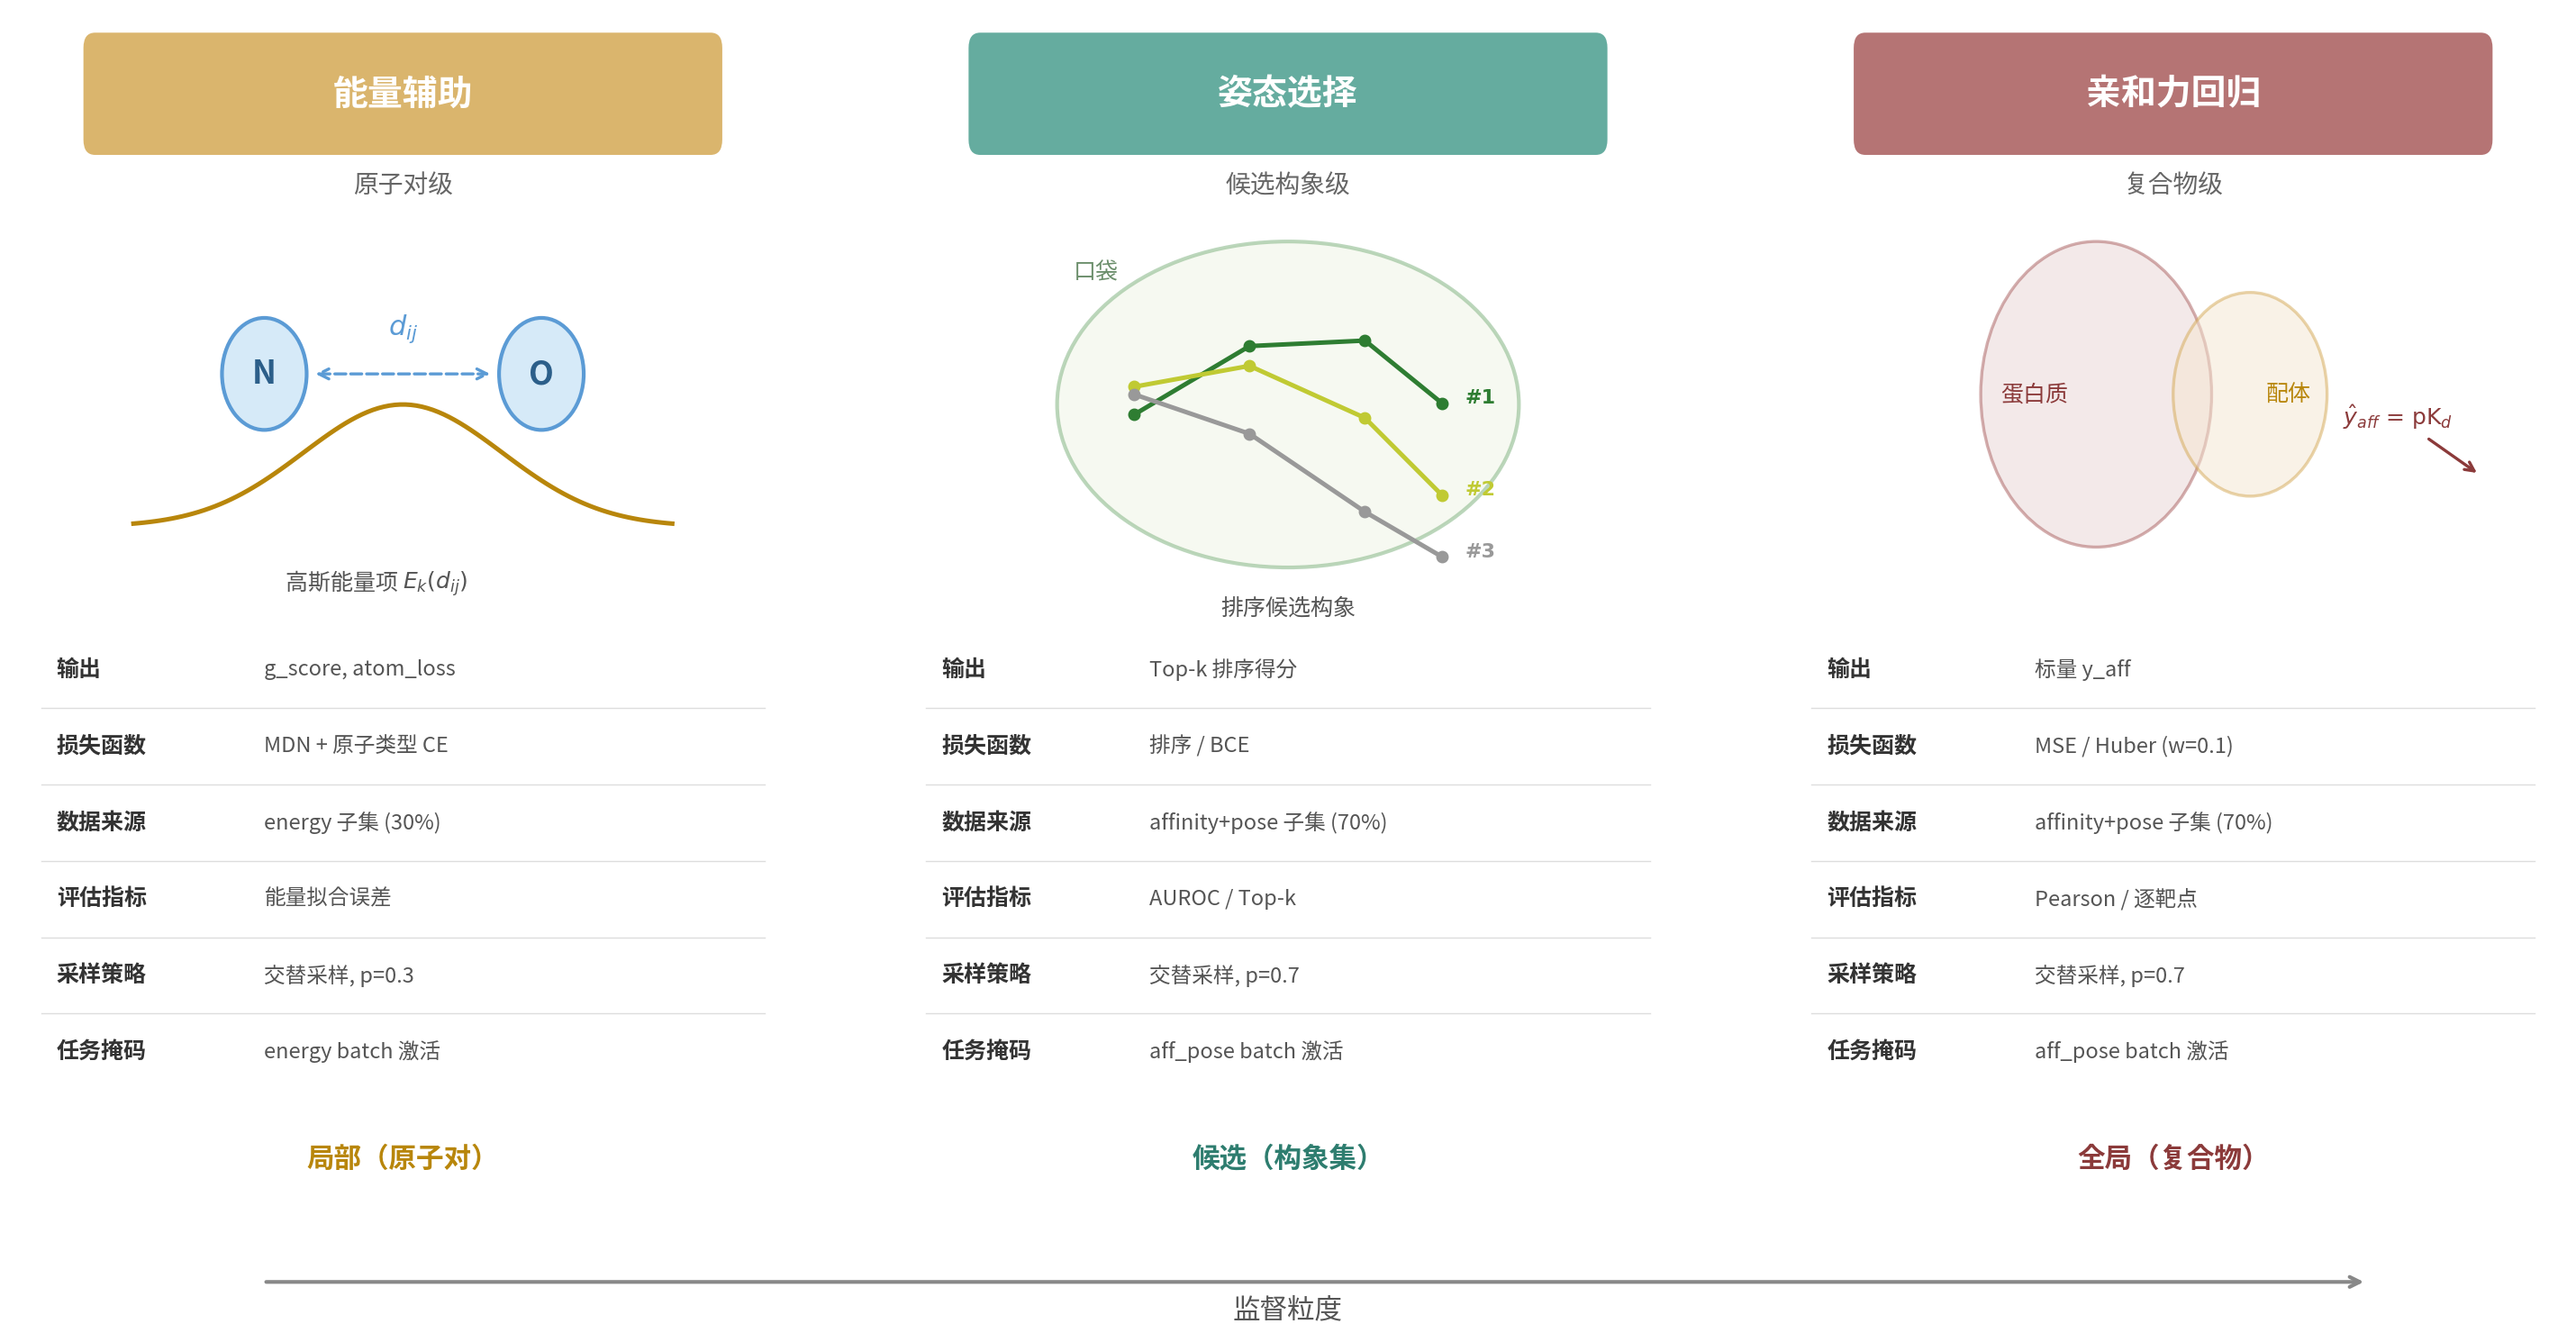
\includegraphics[width=0.92\textwidth]{images/task_comparison.png}
  \caption{InterMoBA-MTL 三类任务的监督粒度、输入语境与输出形式对比示意。由左至右监督粒度从原子对级放大到复合物级，对应局部—候选—全局三层语义递进关系。}
  \label{F.task_comparison}
\end{figure}

从表~\ref{T.task_comparison} 与图~\ref{F.task_comparison} 可以看到，三类任务构成一条清晰的语义层次链：能量辅助监督作用在最细的原子对粒度上，姿态选择在候选构象集合上做相对判别，亲和力回归则在整个复合物上给出全局打分。这种“局部—候选—全局”的层次关系不仅解释了为何不能把它们简单加和为单一 loss，也构成了本文课程学习按“先局部、后全局”引入任务的直接动机。

在工程实现上，本文将多任务前向统一为五输出契约，使得一次 forward 即可同时产生上述三类任务所需的全部结果，而是否参与当前 batch 的损失计算由 \texttt{task\_mask} 决定。该设计避免了任务头互斥带来的训练分支割裂，使亲和力、姿态和能量监督能够在同一共享表示空间内被一致优化和评估。

\subsection{多尺度联合监督的理论依据与机制分析}

把这三类任务放在一起训练不只是工程上的便利，背后有几条相互关联的理论线索可以解释为什么联合训练有望带来更好的预测性能。下面分五个角度展开。

\textbf{（1）辅助任务带来的隐式正则化。}经典多任务理论认为，辅助任务会给共享表示施加归纳偏置（inductive bias），让模型偏向那些能同时解释多个任务的假设空间\cite{caruana1997multitask,ruder2017overview}。放到本文的场景里，能量辅助监督要求共享 Graph-Transformer 编码器必须学到原子对层面的物理特征——范德华距离响应、氢键供受体匹配、疏水接触模式——而这些恰恰是宏观亲和力的微观基础。能量任务虽然不直接参加亲和力评测，但它约束了共享表示的学习方向，相当于一种正则化，能减少模型对训练集中特定蛋白统计偏差的过拟合。

\textbf{（2）多尺度监督的互补性。}三类任务形成原子对级（能量）$\rightarrow$ 构象级（姿态选择）$\rightarrow$ 复合物级（亲和力）的层次化监督。类似的思路在 AlphaFold 2 中也有体现：FAPE、distogram、pLDDT 等中间辅助目标帮助模型学到更稳定的结构表征\cite{jumper2021highly}。如果只训练亲和力回归，模型很容易走捷径——靠口袋体积、配体分子量等全局描述符给一个粗糙的预测，碰到分布外靶点就不可靠。加了原子对级能量监督之后，模型不得不去理解结合亲和力背后的物理成因，内部表征也就更有物理一致性。

\textbf{（3）物理约束有助于面对新靶点。}训练集和测试集的靶点分布差异是蛋白质-配体预测绕不开的难题。PIGNet 把结合自由能拆成范德华、氢键、金属配位和疏水等物理分量，在未见靶点上展现了更稳健的泛化；PIGNet2 在 DUD-E 虚拟筛选基准上再次证实了这一点\cite{moon2022pignet,moon2024pignet2}。本文 $g\_score$ 的四分量高斯能量建模和 PIGNet 系列的物理分解思路方向一致：把打分函数的学习过程锚定在可解释的物理相互作用模式上，减少模型对训练集中特定蛋白-配体对的记忆依赖，在分布外（out-of-distribution）场景下维持更可靠的预测。

\textbf{（4）姿态判别和亲和力预测相互促进。}GNINA 的实验发现，把亲和力预测和 pose 质量判别一起优化能提升虚拟筛选的富集效果\cite{mcnutt2021gnina}。道理不难理解：亲和力预测的前提是输入构象得对，而 pose 排序帮助模型分辨真正的原子接触模式、过滤对接采样引入的几何噪声，给亲和力预测提供更干净的结构输入。在本文的双数据源交替训练中，affinity+pose 数据源同时携带亲和力标签和 pose 质量标签，模型一边判别构象质量一边学全局打分，两个任务互相为对方提供有用的信号。

\textbf{（5）固定权重的简洁与可控。}怎样平衡多任务损失一直是联合训练的难点。不确定性加权\cite{kendall2018multi}和 DWA\cite{liu2019end} 等自适应方法虽然灵活，但引入了额外可学习参数或历史依赖，训练早期有时不够稳定。本文主实验选择了更简单的固定权重策略——按各任务损失的量级预设加权系数，训练行为完全可复现，也方便做消融。这个选择之所以行得通，是因为预训练阶段只有亲和力和姿态两个量级相近的任务，不需要复杂的自适应调节；微调阶段虽然加了量级较小的能量监督，但主干冻结和渐进解冻已经隔离了新旧任务间的梯度干扰，固定权重就够用了。

以上五个角度各有独立的文献依据\cite{caruana1997multitask,jumper2021highly,moon2022pignet,mcnutt2021gnina}，本文做的事情是把它们拼合到蛋白质-配体建模这个具体场景中，用一套统一的工程框架实现联合训练、联合评测和联合消融。

\subsection{多任务损失加权与双数据源数据流}

\subsubsection{损失加权策略}

多任务训练绕不开的一个问题是怎样把量纲、分布和收敛速度不同的多个损失合并为一个优化目标\cite{chen2018gradnorm}。本文在损失层实现了三种可切换的加权策略。

\textbf{固定权重策略（Fixed）}是本文主实验采用的方法，将预设的静态权重 $w_t$ 直接应用于各任务损失：

\begin{equation}
\mathcal{L}_{total}^{fixed} = \sum_{t \in \mathcal{T}} w_t \cdot \mathcal{L}_t
\label{eq:loss_fixed}
\end{equation}

该策略与上游 Interformer\cite{lai2024interformer}的默认行为一致，简单稳定且完全可复现。其局限在于权重 $w_t$ 需手工设定，无法适应训练中各任务 loss 的动态变化。作为备选，系统还实现了同方差不确定性加权（通过可学习参数 $s_t = \log \sigma_t^2$ 自动调节任务权重）\cite{kendall2018multi}和动态权重平均 DWA（根据相邻 epoch 的 loss 下降率动态分配权重）\cite{liu2019end}两种自适应策略。表~\ref{T.strategy_comparison} 对比了三者的核心差异。

\begin{table}[htb]
  \centering
  \caption{三种多任务损失加权策略的对比}
  \label{T.strategy_comparison}
  \small
  \begin{tabular}{p{2.2cm}p{3.0cm}p{3.2cm}p{3.0cm}}
    \toprule
    策略 & 可学习参数 & 核心优势 & 适用条件 \\
    \midrule
    Fixed & 无 & 可复现性强，调参直观 & 任务 loss 量级已知且稳定 \\
    Uncertainty\cite{kendall2018multi} & $s_t = \log \sigma_t^2$ & 自动平衡异质 loss & 回归与分类混合场景 \\
    DWA\cite{liu2019end} & 无（依赖 loss 历史） & 动态追踪训练难度 & Epoch 级调整即可 \\
    \bottomrule
  \end{tabular}
\end{table}

在所有策略中，最终的总损失还需与训练阶段门控系数 $m_t \in [0, 1]$ 串联，并附加几何约束项：

\begin{equation}
\mathcal{L}_{final} = \sum_{t \in \mathcal{T}} m_t \cdot \lambda_t \cdot \mathcal{L}_t \;+\; 0.1 \cdot (\mathcal{L}_{collision} + \mathcal{L}_{min\_dist})
\label{eq:loss_final}
\end{equation}

其中，$\lambda_t$ 由所选加权策略决定（公式~\ref{eq:loss_fixed}及表~\ref{T.strategy_comparison}），$m_t$ 按训练阶段输出（详见下一小节），$\mathcal{L}_{collision}$ 和 $\mathcal{L}_{min\_dist}$ 为原子对级几何约束，以固定系数附加，用于惩罚原子碰撞和违反范德华半径下界的构象。这种串联设计使得训练阶段控制（"何时激活任务"）与权重平衡（"激活后梯度占比"）在职责上互不干扰\cite{zhang2021survey}。

\subsubsection{双数据源交替采样机制}

多任务训练还面临数据异构的问题：energy 监督来自对接构象的分子间能量标注，affinity+pose 监督来自实验测定的结合亲和力和 pose 质量标签，两套数据在样本语义、标注形式和预处理路径上都不同。这类部分标注（partial annotation）问题在药物发现\cite{wu2018moleculenet}和多任务学习\cite{zhang2021survey}中并不少见，常见做法是对缺失标注做掩蔽而不是硬填伪标签。

本文采用 \textbf{batch 级任务掩蔽与概率加权交替采样}策略。系统分别构造 energy 和 affinity+pose 两个独立 DataLoader，通过自定义交替迭代器按预设概率 $p$ 在二者间做加权随机轮询。每个采样到的 batch 携带 \texttt{task\_id}（标识数据来源）和 \texttt{task\_mask}（指定当前 batch 应计算哪些任务的损失）。表~\ref{T.task_mask} 给出了两种数据源对应的任务掩蔽矩阵。

\begin{table}[htb]
  \centering
  \caption{双数据源的任务掩蔽矩阵（1=计算损失并反传梯度，0=掩蔽）}
  \label{T.task_mask}
  \small
  \begin{tabular}{lccccc}
    \toprule
    数据源（采样概率） & 亲和力 & 姿态选择 & $g\_score$ & $g\_score\_pos$ & 原子类型 \\
    \midrule
    Energy ($p=0.3$) & 0 & 0 & 1 & 1 & 1 \\
    Affinity+Pose ($p=0.7$) & 1 & 1 & 0 & 0 & 0 \\
    \bottomrule
  \end{tabular}
\end{table}

一个训练 epoch 的总步数等于两个子 DataLoader 的 batch 数之和（max-size-cycle 语义）。当较小的数据源提前耗尽时，采样器自动循环重启以维持比例，直到较大的数据源也完成一轮遍历。默认采样概率 $p_{energy} = 0.3$，即约 30\% 的训练步用于能量监督，70\% 用于亲和力与姿态监督，该比例可作为超参数在消融实验中调整。

这套设计有三点好处。第一，每个 batch 内部只有单一任务，不存在样本级混合带来的梯度干扰\cite{yu2020gradient}。第二，被掩蔽的任务头只做前向计算不回传梯度（loss 乘 0 后 \texttt{detach()}），统一输出契约的完整性保留了，也不会引入虚假监督。第三，训练主循环只要根据 \texttt{task\_mask} 决定计算哪些损失就行，和上游单任务代码完全兼容，框架改动很小。

\subsection{两阶段训练策略与 MoBA 任务敏感路由}

\subsubsection{预训练—微调的两阶段训练策略}

训练分两个阶段。第一阶段只用 affinity+pose 数据训练共享 Graph-Transformer 主干、亲和力头和姿态选择头，让模型先学到稳定的蛋白质-配体交互表示。第二阶段加载预训练参数后加入能量任务头，通过双数据源交替采样把 energy 监督接进来。

微调初期先冻住 backbone，只更新新加的任务头和输出层参数；等能量分支初步适配后再渐进解冻共享主干，做端到端联合优化。这样做的目的是防止随机初始化的能量头在训练早期用大梯度冲坏预训练表示，也能保留亲和力和姿态任务已经学好的全局判别能力。

简单说，预训练解决“怎样拿到可靠的共享表示”，微调解决“怎样在不破坏已有能力的前提下加入局部物理监督”。这和本文任务的“局部—候选—全局”监督层次是匹配的：先用亲和力和姿态任务打好全局判别基础，再通过能量辅助监督补强局部相互作用建模。表~\ref{T.two_stage_summary} 总结了两阶段的任务激活状态和设计动机。

\begin{table}[hbt]
  \centering
  \caption{两阶段训练策略的任务激活设计}
  \label{T.two_stage_summary}
  \small
  \begin{tabular}{lcccp{5.5cm}}
    \toprule
    阶段 & 能量任务 & 姿态选择 & 亲和力 & 设计动机 \\
    \midrule
    预训练 & $\times$ & $\checkmark$ & $\checkmark$ & 建立稳定的结构表示与全局判别能力 \\
    微调（冻结期） & $\checkmark$ & $\checkmark$ & $\checkmark$ & 安全引入能量监督，保护预训练表示 \\
    微调（解冻期） & $\checkmark$ & $\checkmark$ & $\checkmark$ & 全任务端到端联合优化 \\
    \bottomrule
  \end{tabular}
\end{table}

\subsubsection{任务敏感路由与节点级 MoBA 融合}

除两阶段训练策略外，本文还对多任务场景下的计算路径进行了任务敏感路由。MoBA 适配层在多任务框架中默认配置为 \texttt{energy\_only} 模式：\texttt{task\_id = energy} 的批次进入局部稀疏增强路径；亲和力与姿态批次绕过该路径，使用标准共享编码流。这一设计源于两类任务对表示需求的本质差异：能量相关监督高度依赖局部原子对的几何精度，MoBA 的块稀疏注意力机制可有效捕获短程密集交互；而亲和力与 pose 排序更依赖稳定的跨片段全局上下文，全局稠密注意力更为适合\cite{lu2025moba,ying2021transformers}。路由策略可通过 \texttt{moba\_routing} 参数在 \texttt{all}、\texttt{energy\_only} 和 \texttt{off} 三种模式间切换。

\textbf{节点级单路融合机制。}在 MoBA 适配层内部，本文采用\textbf{仅更新节点特征、边特征直通}的单路融合设计。MoBA 适配器对节点表示 $h_{node}$ 施加块稀疏局部注意力后输出增强节点表示 $\hat{h}_{node}$，随即通过门控残差 MLP 与原始节点表示拼接融合：

\begin{equation}
h_{node}^{\prime} = f_{node}\!\left(\left[\hat{h}_{node} \,\|\, h_{node}\right]\right), \quad h_{edge}^{\prime} = h_{edge}
\label{eq:moba_node_fuse}
\end{equation}

其中 $f_{node}(\cdot)$ 为 \texttt{mlp\_node\_fuse}，由 LayerNorm $\rightarrow$ Dropout $\rightarrow$ Linear($2d \to d$) $\rightarrow$ ReLU $\rightarrow$ Dropout $\rightarrow$ Linear($d \to d$) $\rightarrow$ LayerNorm 串联构成，将拼接后的 $2d$ 维向量映射回原始维度 $d$；$[\cdot \| \cdot]$ 表示通道维拼接。

\begin{table}[htb]
  \centering
  \caption{MoBA 节点级单路融合机制：节点与边特征的处理策略}
  \label{T.moba_fusion}
  \small
  \begin{tabular}{p{2.8cm}p{2.2cm}p{3.0cm}p{3.6cm}}
    \toprule
    特征流 & 是否经 MoBA & 融合操作 & 设计依据 \\
    \midrule
    节点特征 $h_{node}$ & 是 & MLP 门控残差融合 & 承载可学习语义状态，需引入局部稀疏增强 \\
    边特征 $h_{edge}$ & 否（直通） & 无 & 编码分子几何先验，不宜被稀疏注意力扰动 \\
    \bottomrule
  \end{tabular}
\end{table}

这样设计的理由是 Graph Transformer 中节点和边的职责本来就不同\cite{ying2021transformers}：节点表示承载原子/残基级的语义状态，适合用注意力更新；边特征编码的是键合类型、原子对距离等结构化几何先验，在输入端就已经固化，经稀疏注意力扰动反而会破坏几何约束\cite{lai2024interformer}。另外，单路融合只需维护 \texttt{mlp\_node\_fuse} 一组参数，去掉了 \texttt{moba\_edge\_norm} 和 \texttt{mlp\_edge\_fuse}，在大批量多任务训练中能降低显存峰值。

\newpage

\section{能量监督与可解释性约束}
\subsection{四分量高斯能量项}

能量监督沿用了现有系统中的四分量高斯项，思路是用一组参数化高斯函数来近似不同距离区间的局部相互作用。这类做法在分子力场设计中很常见，AutoDock Vina\cite{trott2010autodock} 的打分函数也是用高斯型项来近似范德华和氢键作用。形式上可写为：

\begin{equation}
 E(d) = \sum_{k=1}^{4} w_k \cdot \exp\left(-\frac{(d - \mu_k)^2}{2\sigma_k^2}\right)
\end{equation}

其中，$d$ 为原子对表面距离，$w_k$、$\mu_k$ 和 $\sigma_k$ 分别表示第 $k$ 个分量的权重、中心和宽度。该设计并非将模型等同于严格物理模拟器，而是为局部原子对相互作用提供可解释的辅助监督形式。

从语义上看，这四个分量可分别对应近距离排斥、范德华吸引、疏水作用和氢键相关作用。图~\ref{F.gaussian_components} 展示了高斯分量的响应分布示意，它更适合作为方法解释和案例分析的辅助图，而不是独立的最终 benchmark 结论。

\begin{figure}[hbt]
  \centering
  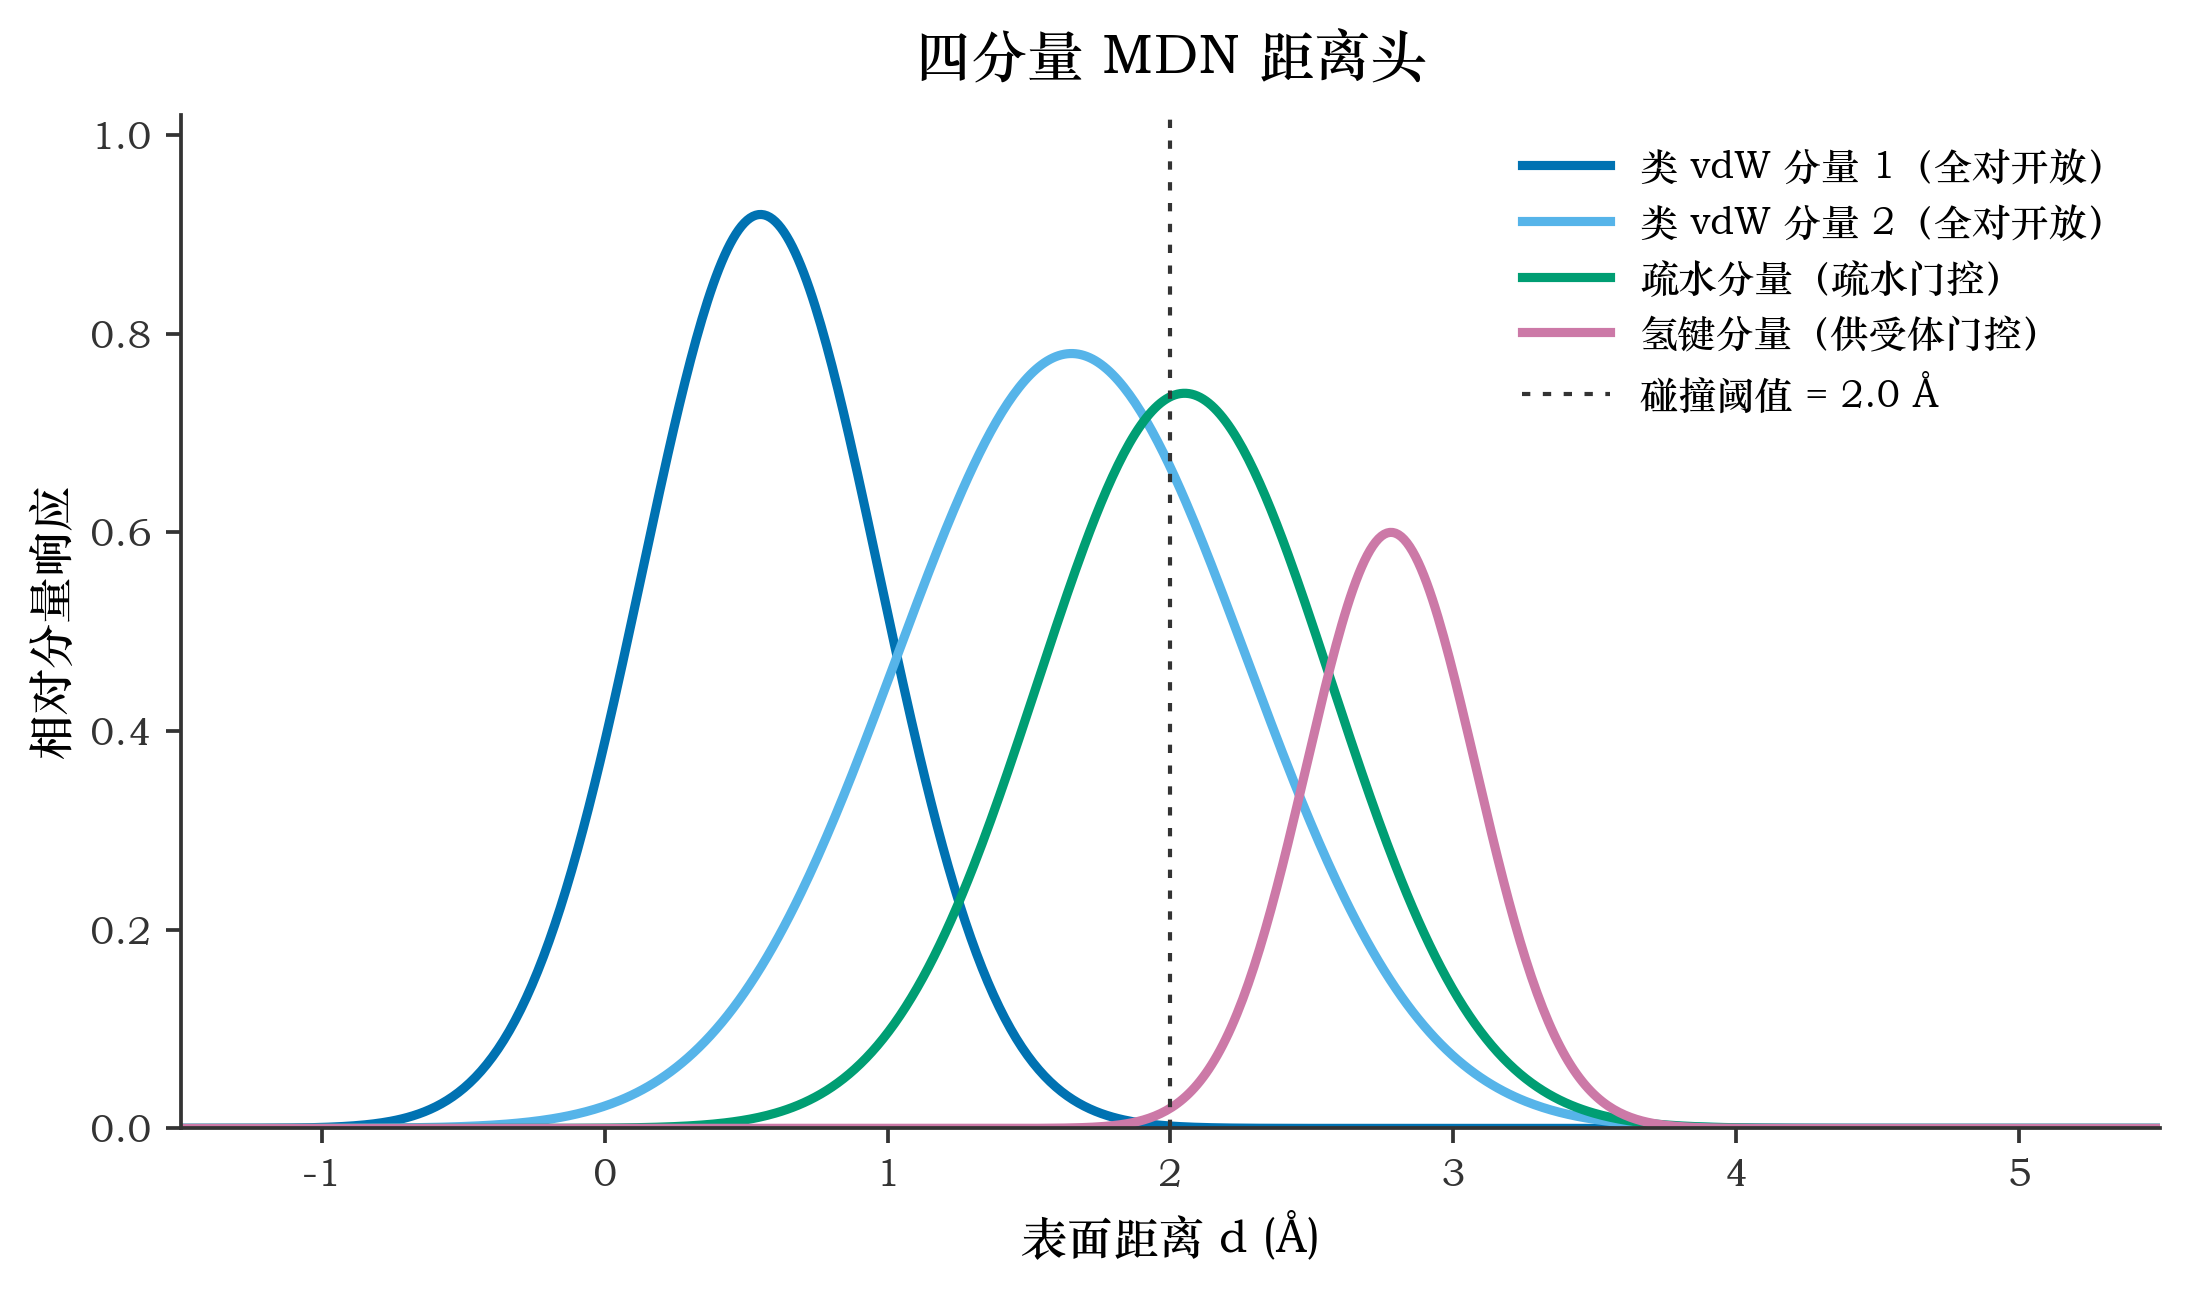
\includegraphics[width=0.78\textwidth]{images/gaussian_components.png}
  \caption{四分量高斯能量项分布示意}
  \label{F.gaussian_components}
\end{figure}

\subsection{原子对类型掩蔽机制}

为了保证能量相关项不会在明显不合理的原子对上被错误激活，系统引入了原子对类型掩蔽机制：

\begin{equation}
 E_{ij}(d) = \sum_{k=1}^{4} m_{ij}^{(k)} \cdot w_k \cdot \exp\left(-\frac{(d - \mu_k)^2}{2\sigma_k^2}\right)
\end{equation}

其中，$m_{ij}^{(k)} \in \{0,1\}$ 表示原子对 $(i,j)$ 是否允许参与第 $k$ 类相互作用。通过这种显式掩蔽，可以使疏水项主要作用于非极性原子对，使氢键项更多约束供体-受体匹配关系，而不是将所有作用都无差别地叠加到全部原子对上。

\subsection{几何约束与能量分解可视化}

除类型掩蔽外，系统还通过简单几何约束提升局部监督的物理合理性。例如，原子对距离不应持续违反范德华半径下界，氢键相关作用也需要满足一定的空间条件。这类约束虽然无法替代高精度物理模拟，但能够有效减少明显不合理的训练信号。

总能量可被分解为若干局部项：

\begin{equation}
 E_{total} = E_{repulsion} + E_{vdW} + E_{hydrophobic} + E_{hbond}
\end{equation}

图~\ref{F.energy_decomposition} 给出了能量分解的可视化结果。这些能量响应可以看出四分量高斯项在哪些空间位置比较活跃，进一步做归因聚合还可以把解释信号分配到配体原子层面。本文主要拿它们做案例分析，看模型输出是不是和氢键、疏水接触位点等化学常识匹配，为先导化合物优化提供一些物理层面的参考。

\begin{figure}[hbt]
  \centering
  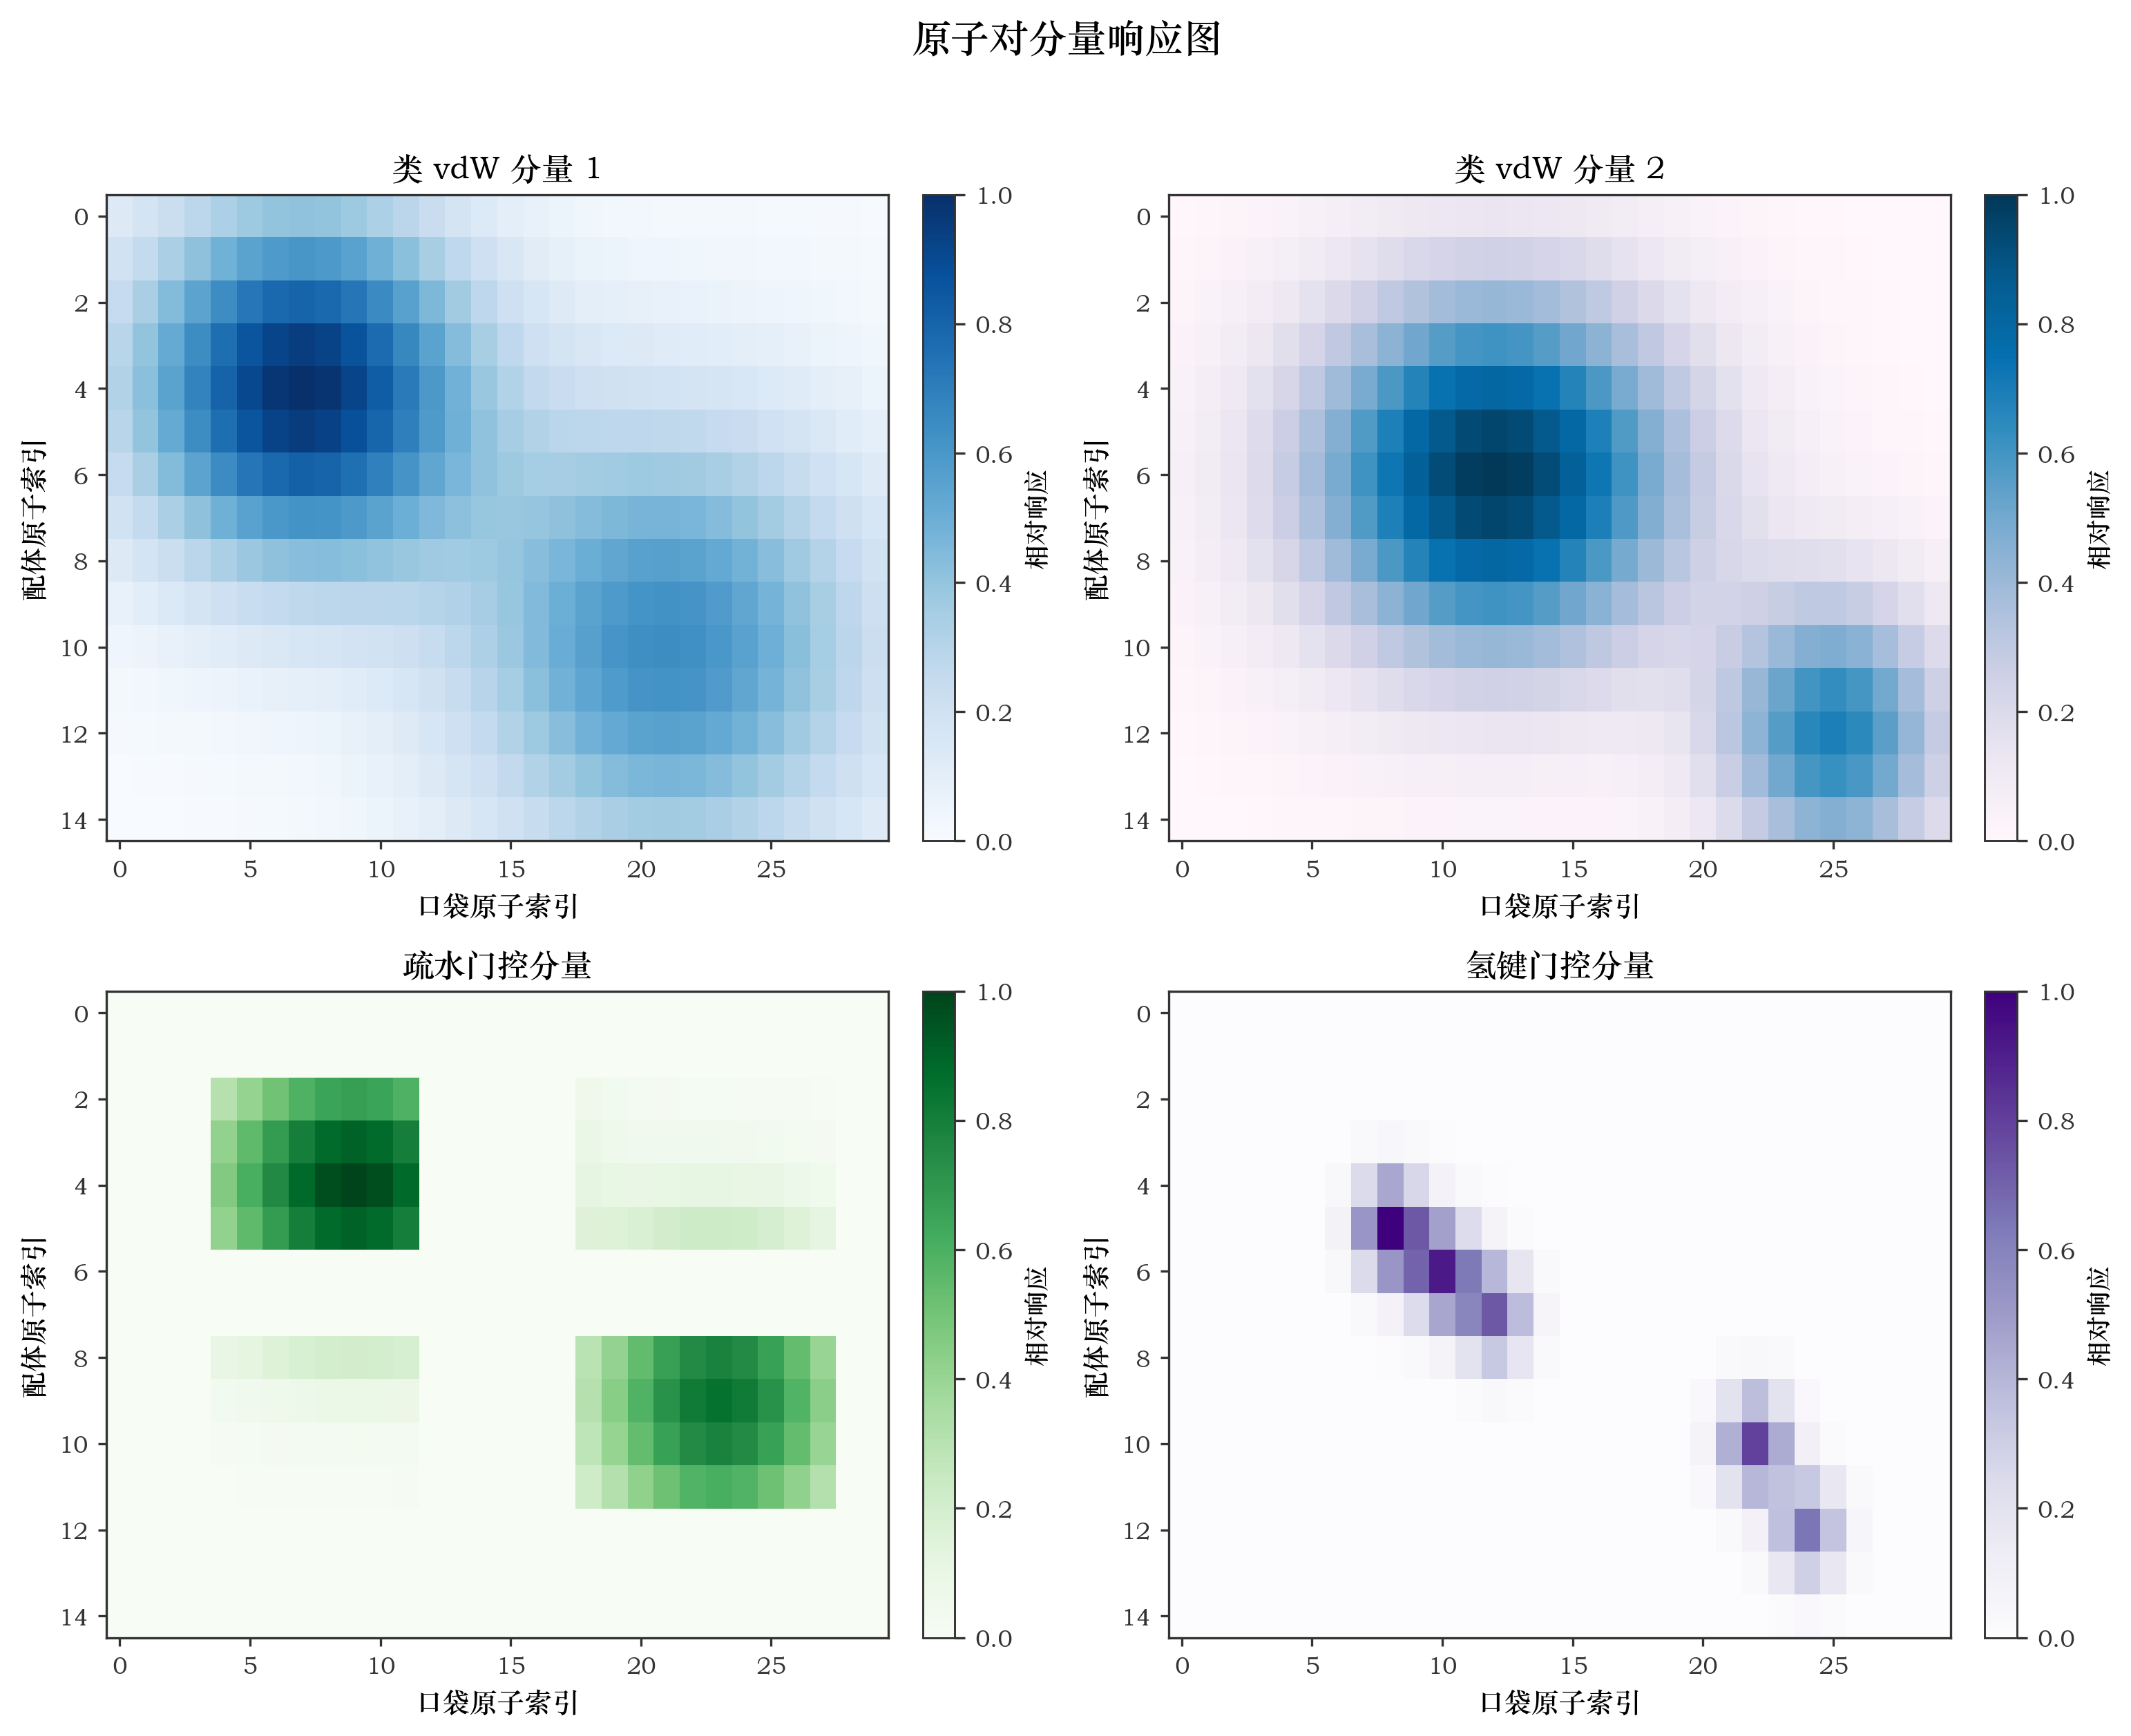
\includegraphics[width=0.8\textwidth]{images/energy_decomposition.png}
  \caption{四分量混合头的原子对级响应示意。四个子图分别对应两个 \texttt{vdW-like} 分量、疏水门控分量与氢键门控分量；颜色表示 mixture 中的相对响应强弱，用于展示局部解释信号的空间分布。}
  \label{F.energy_decomposition}
\end{figure}

\newpage

\section{评测协议}
\subsection{评测场景与模型角色}

InterMoBA-MTL 的核心角色是\textbf{候选构象重排序与亲和力打分}，而非替代传统对接软件的构象搜索过程。评测时，候选 pose 由上游对接引擎（如 GNINA\cite{mcnutt2021gnina}）预先生成，模型对其进行打分排序并输出亲和力预测值。因此，本文的评测协议围绕以下两个场景展开：

（1）\textbf{PDBbind time-split 测试集}（341 targets，7161 poses）：评估模型在训练数据分布内（但时间上严格隔离）的亲和力预测与姿态选择性能；

（2）\textbf{PoseBusters Benchmark v2}\cite{buttenschoen2024posebusters}（308 个复合物，均沉积于 2021 年后）：评估模型在训练分布外的独立数据上的对接精度与物理合理性。

\subsection{评测指标}

本文实验中实际报告的指标分为以下三组：

\textbf{亲和力预测指标}：Pearson 相关系数 $R$、Spearman 秩相关系数 $\rho$ 和均方根误差 RMSE。评估在两个口径下进行：全量 crystal pose（$n=341$）和 pIC50 $> 0.1$ 子集（$n=204$）。

\textbf{姿态选择指标}：AUROC 和 Top-$k$ 成功率（$k=1,3,5$）。Top-$k$ 成功率定义为：

\begin{equation}
 \text{Top-K Success Rate} = \frac{1}{N}\sum_{i=1}^{N}\mathbb{I}\left[\min_{k \leq K}\text{RMSD}(P_i^{(k)}, P_i^{ref}) < \delta\right]
\end{equation}

其中，$P_i^{(k)}$ 表示第 $i$ 个复合物经模型排序后的第 $k$ 个候选姿态，$P_i^{ref}$ 为参考晶体构象，$\delta = 2\,\text{\AA}$。Pearson 相关系数为：

\begin{equation}
 r = \frac{\sum_{i=1}^{N}(y_i - \bar{y})(\hat{y}_i - \bar{\hat{y}})}{\sqrt{\sum_{i=1}^{N}(y_i - \bar{y})^2}\sqrt{\sum_{i=1}^{N}(\hat{y}_i - \bar{\hat{y}})^2}}
\end{equation}

\textbf{独立基准指标}（PoseBusters Benchmark v2）：RMSD$<2$\,\AA{} 成功率和 PB-valid 比例。PB-valid 要求 pose 同时满足 RMSD$<2$\,\AA{} 并通过键长、键角、位阻、芳香环平面性等 20 余项物理合理性检查。

\subsection{辅助分析指标}

除上述量化指标外，本文还从两个维度补充分析：

（1）\textbf{相互作用恢复率}：使用 PLIP\cite{adasme2021plip} 对晶体结构和模型 Top-1 预测 pose 分别提取氢键与疏水接触，计算恢复比例，用于评估排序靠前的 pose 是否保留了关键非共价相互作用。

（2）\textbf{训练过程诊断}：训练中记录的分任务损失曲线、多任务权重（\texttt{mtl\_weight}）和梯度范数等日志信息，用于说明多任务机制的运行状态，不作为模型性能的评判依据。

\newpage

\section{实验与分析}
\subsection{实验设置}
\subsubsection{数据组织}

数据不是一个静态张量文件，而是由 CSV 索引表、结构文件和 LMDB 缓存三部分组成。所有数据来自 PDBbind 2020 General Set，按 time-split 协议划分后根据任务角色拆成两个子集。表~\ref{T.dataset} 列出了各数据资产的样本规模。

\begin{table}[htb]
  \centering
  \caption{实验使用的主要数据资产、样本规模与划分}
  \label{T.dataset}
  \scriptsize
  \setlength{\tabcolsep}{4pt}
  \renewcommand{\arraystretch}{1.2}
  \begin{tabular}{p{2.6cm}p{1.6cm}p{1.6cm}p{1.6cm}p{1.6cm}p{2.8cm}}
  \hline
  数据资产 & 总量 & 训练集 & 验证集 & 测试集 & 说明 \\
  \hline
  Energy 子集 & 19{,}443 & 16{,}379 & 968 & 363 & 每 target 1 条，单 crystal pose \\
  Affinity+Pose 子集 & 392{,}406 & 331{,}527 & 19{,}341 & 7{,}161 & 18{,}686 targets，$\sim$21 poses/target \\
  PoseBusters v2 & 308 & --- & --- & 308 & 独立基准，均沉积于 2021 年后 \\
  \hline
  \end{tabular}
\end{table}

其中，Energy 子集（\texttt{general\_PL\_2020.csv}）包含 19{,}443 个蛋白质-配体复合物，每个 target 对应一条 crystal pose 记录，用于提供能量相关监督信号。Affinity+Pose 子集（\texttt{general\_PL\_2020\_round0\_full.csv}）包含 392{,}406 条 pose 记录，覆盖 18{,}686 个 target，每个 target 平均约 21 个候选构象（含 GNINA 生成的 decoy），用于训练亲和力回归与姿态选择任务。两个子集按 DiffDock time-split 协议统一划分\cite{corso2023diffdock}，测试集包含 363 个 target（其中 341 个在 Affinity+Pose 子集中有有效结构数据，对应 7{,}161 个 poses）。

所有数据来自公开的 PDBbind 数据库\cite{wang2004pdbbind,liu2015pdbbind}，划分遵循 DiffDock 的 time-split 协议\cite{corso2023diffdock}，降低同类靶点或相似配体泄漏带来的乐观偏差。

原始结构文件需要经过预处理才能送进神经网络。如图~\ref{F.data_pipeline} 所示，流程分七个步骤：索引过滤、结构加载、复合体构建、图特征转换、有效性校验、LMDB 缓存写入和 time-split 切分。复合体构建时会同时保留氢键、疏水接触等局部相互作用信息\cite{adasme2021plip}。

在蛋白质口袋准备方面，本文采用两阶段局部化策略\cite{lai2024interformer,mcnutt2021gnina}：首先以参考配体为中心截取局部口袋并通过残基扩展机制保留完整残基的化学环境；随后在图构建时以 10\,\AA{} 距离阈值进一步筛选蛋白原子，在覆盖关键结合环境与控制图规模之间取得平衡。图~\ref{F.pocket_preparation_placeholder} 以 PDB 3w2o 为例展示了该策略的效果。

\begin{figure}[htb]
  \centering
  \resizebox{0.52\textwidth}{!}{% TikZ 数据预处理流程图（Nature 风格）
% 配色: Wong (Nature Methods, 2011) 色盲安全调色板
% 布局: 水平流水线 + 纵向分支，简洁克制
\begin{tikzpicture}[
    font=\small,
    node distance=3mm and 6mm,
]

% Wong 调色板
\definecolor{wongBlue}{HTML}{0072B2}
\definecolor{wongSkyBlue}{HTML}{56B4E9}
\definecolor{wongGreen}{HTML}{009E73}
\definecolor{wongOrange}{HTML}{E69F00}
\definecolor{wongVermillion}{HTML}{D55E00}
\definecolor{wongRedPurple}{HTML}{CC79A7}

% 淡色填充
\definecolor{tintBlue}{HTML}{DCE8F4}
\definecolor{tintGreen}{HTML}{DFF0E8}
\definecolor{tintOrange}{HTML}{FDF2DC}
\definecolor{tintVermillion}{HTML}{F8E5D6}
\definecolor{tintSky}{HTML}{E4F0F9}
\definecolor{tintRP}{HTML}{F3E4ED}

% 节点样式
\tikzset{
    pipenode/.style={
        rounded corners=2pt, draw=#1, line width=0.6pt, fill=#1!8,
        minimum width=28mm, minimum height=10mm,
        align=center, inner sep=2.5pt, font=\small
    },
    pipenode/.default=wongBlue,
    iobox/.style={
        rounded corners=2pt, draw=#1, line width=0.5pt, fill=#1!6,
        minimum width=24mm, minimum height=8mm,
        align=center, inner sep=2pt, font=\footnotesize
    },
    iobox/.default=wongSkyBlue,
    arrow/.style={
        -{Latex[length=1.8mm, width=1.6mm]}, line width=0.55pt, black!70
    },
    phaselabel/.style={
        font=\footnotesize\bfseries, text=black!70
    },
}

% ---- 输入源（顶部两个） ----
\node[iobox=wongSkyBlue] (csv) {CSV 索引表};
\node[iobox=wongSkyBlue, right=28mm of csv] (struct) {PDB / SDF\\结构文件};

% ---- Stage 1: 索引读取与过滤 ----
\node[pipenode=wongBlue, below=8mm of $(csv)!0.5!(struct)$] (s1)
    {索引读取与过滤\\[-1pt]{\footnotesize \texttt{filter\_df}}};

% ---- Stage 2: 结构批量加载 ----
\node[pipenode=wongBlue, below=8mm of s1] (s2)
    {结构批量加载\\[-1pt]{\footnotesize \texttt{read\_pocket} · \texttt{sdf\_load}}};

% ---- Stage 3: 复合体构建 ----
\node[pipenode=wongGreen, below=8mm of s2] (s3)
    {复合体构建\\[-1pt]{\footnotesize \texttt{merge\_sdf\_pdb}}};

% ---- Stage 4: 图特征转换 ----
\node[pipenode=wongGreen, below=8mm of s3] (s4)
    {图特征转换\\[-1pt]{\footnotesize \texttt{complex\_to\_data} · \texttt{pmap\_chunked}}};

% ---- Stage 5: 有效性校验与标签回填 ----
\node[pipenode=wongOrange, below=8mm of s4] (s5)
    {有效性校验\\[-1pt]{\footnotesize \texttt{assign\_label2x}}};

% ---- Stage 6: 数据持久化 ----
\node[pipenode=wongOrange, below=8mm of s5] (s6)
    {LMDB / CSV 缓存写入\\[-1pt]{\footnotesize \texttt{LmdbPPI.make\_shared}}};

% ---- Stage 7: 时间维划分 ----
\node[pipenode=wongVermillion, below=8mm of s6] (s7)
    {时间维划分\\[-1pt]{\footnotesize \texttt{diffdock\_splits}}};

% ---- 输出（底部） ----
\node[iobox=wongRedPurple, below left=8mm and 2mm of s7] (train) {train 子集};
\node[iobox=wongRedPurple, below=8mm of s7] (valid) {valid 子集};
\node[iobox=wongRedPurple, below right=8mm and 2mm of s7] (test) {test 子集};

% ---- 箭头：输入→Stage1 ----
\draw[arrow] (csv.south)   -- (s1.north west);
\draw[arrow] (struct.south) -- (s1.north east);

% ---- 箭头：Stage间 ----
\draw[arrow] (s1) -- (s2);
\draw[arrow] (s2) -- (s3);
\draw[arrow] (s3) -- (s4);
\draw[arrow] (s4) -- (s5);
\draw[arrow] (s5) -- (s6);
\draw[arrow] (s6) -- (s7);

% ---- 箭头：Stage7→输出 ----
\draw[arrow] (s7.south) -- ++(0,-2mm) -| (train.north);
\draw[arrow] (s7.south) -- (valid.north);
\draw[arrow] (s7.south) -- ++(0,-2mm) -| (test.north);

% ---- 右侧阶段标签 ----
\node[phaselabel] at ([xshift=14mm]$(s1.south east)!0.5!(s2.north east)$) {数据准备};
\node[phaselabel] at ([xshift=14mm]$(s3.south east)!0.5!(s4.north east)$) {特征构建};
\node[phaselabel] at ([xshift=14mm]$(s5.south east)!0.5!(s6.north east)$) {质量控制};
\node[phaselabel] at ([xshift=14mm]s7.east) {评测划分};

\end{tikzpicture}
}
  \caption{InterMoBA-MTL 数据预处理流程。七阶段流水线依次完成数据准备（索引过滤与结构加载）、特征构建（复合体合并与图转换）、质量控制（有效性校验与缓存写入）和评测划分（time-split 切分）。}
  \label{F.data_pipeline}
\end{figure}

\begin{figure}[htb]
  \centering
  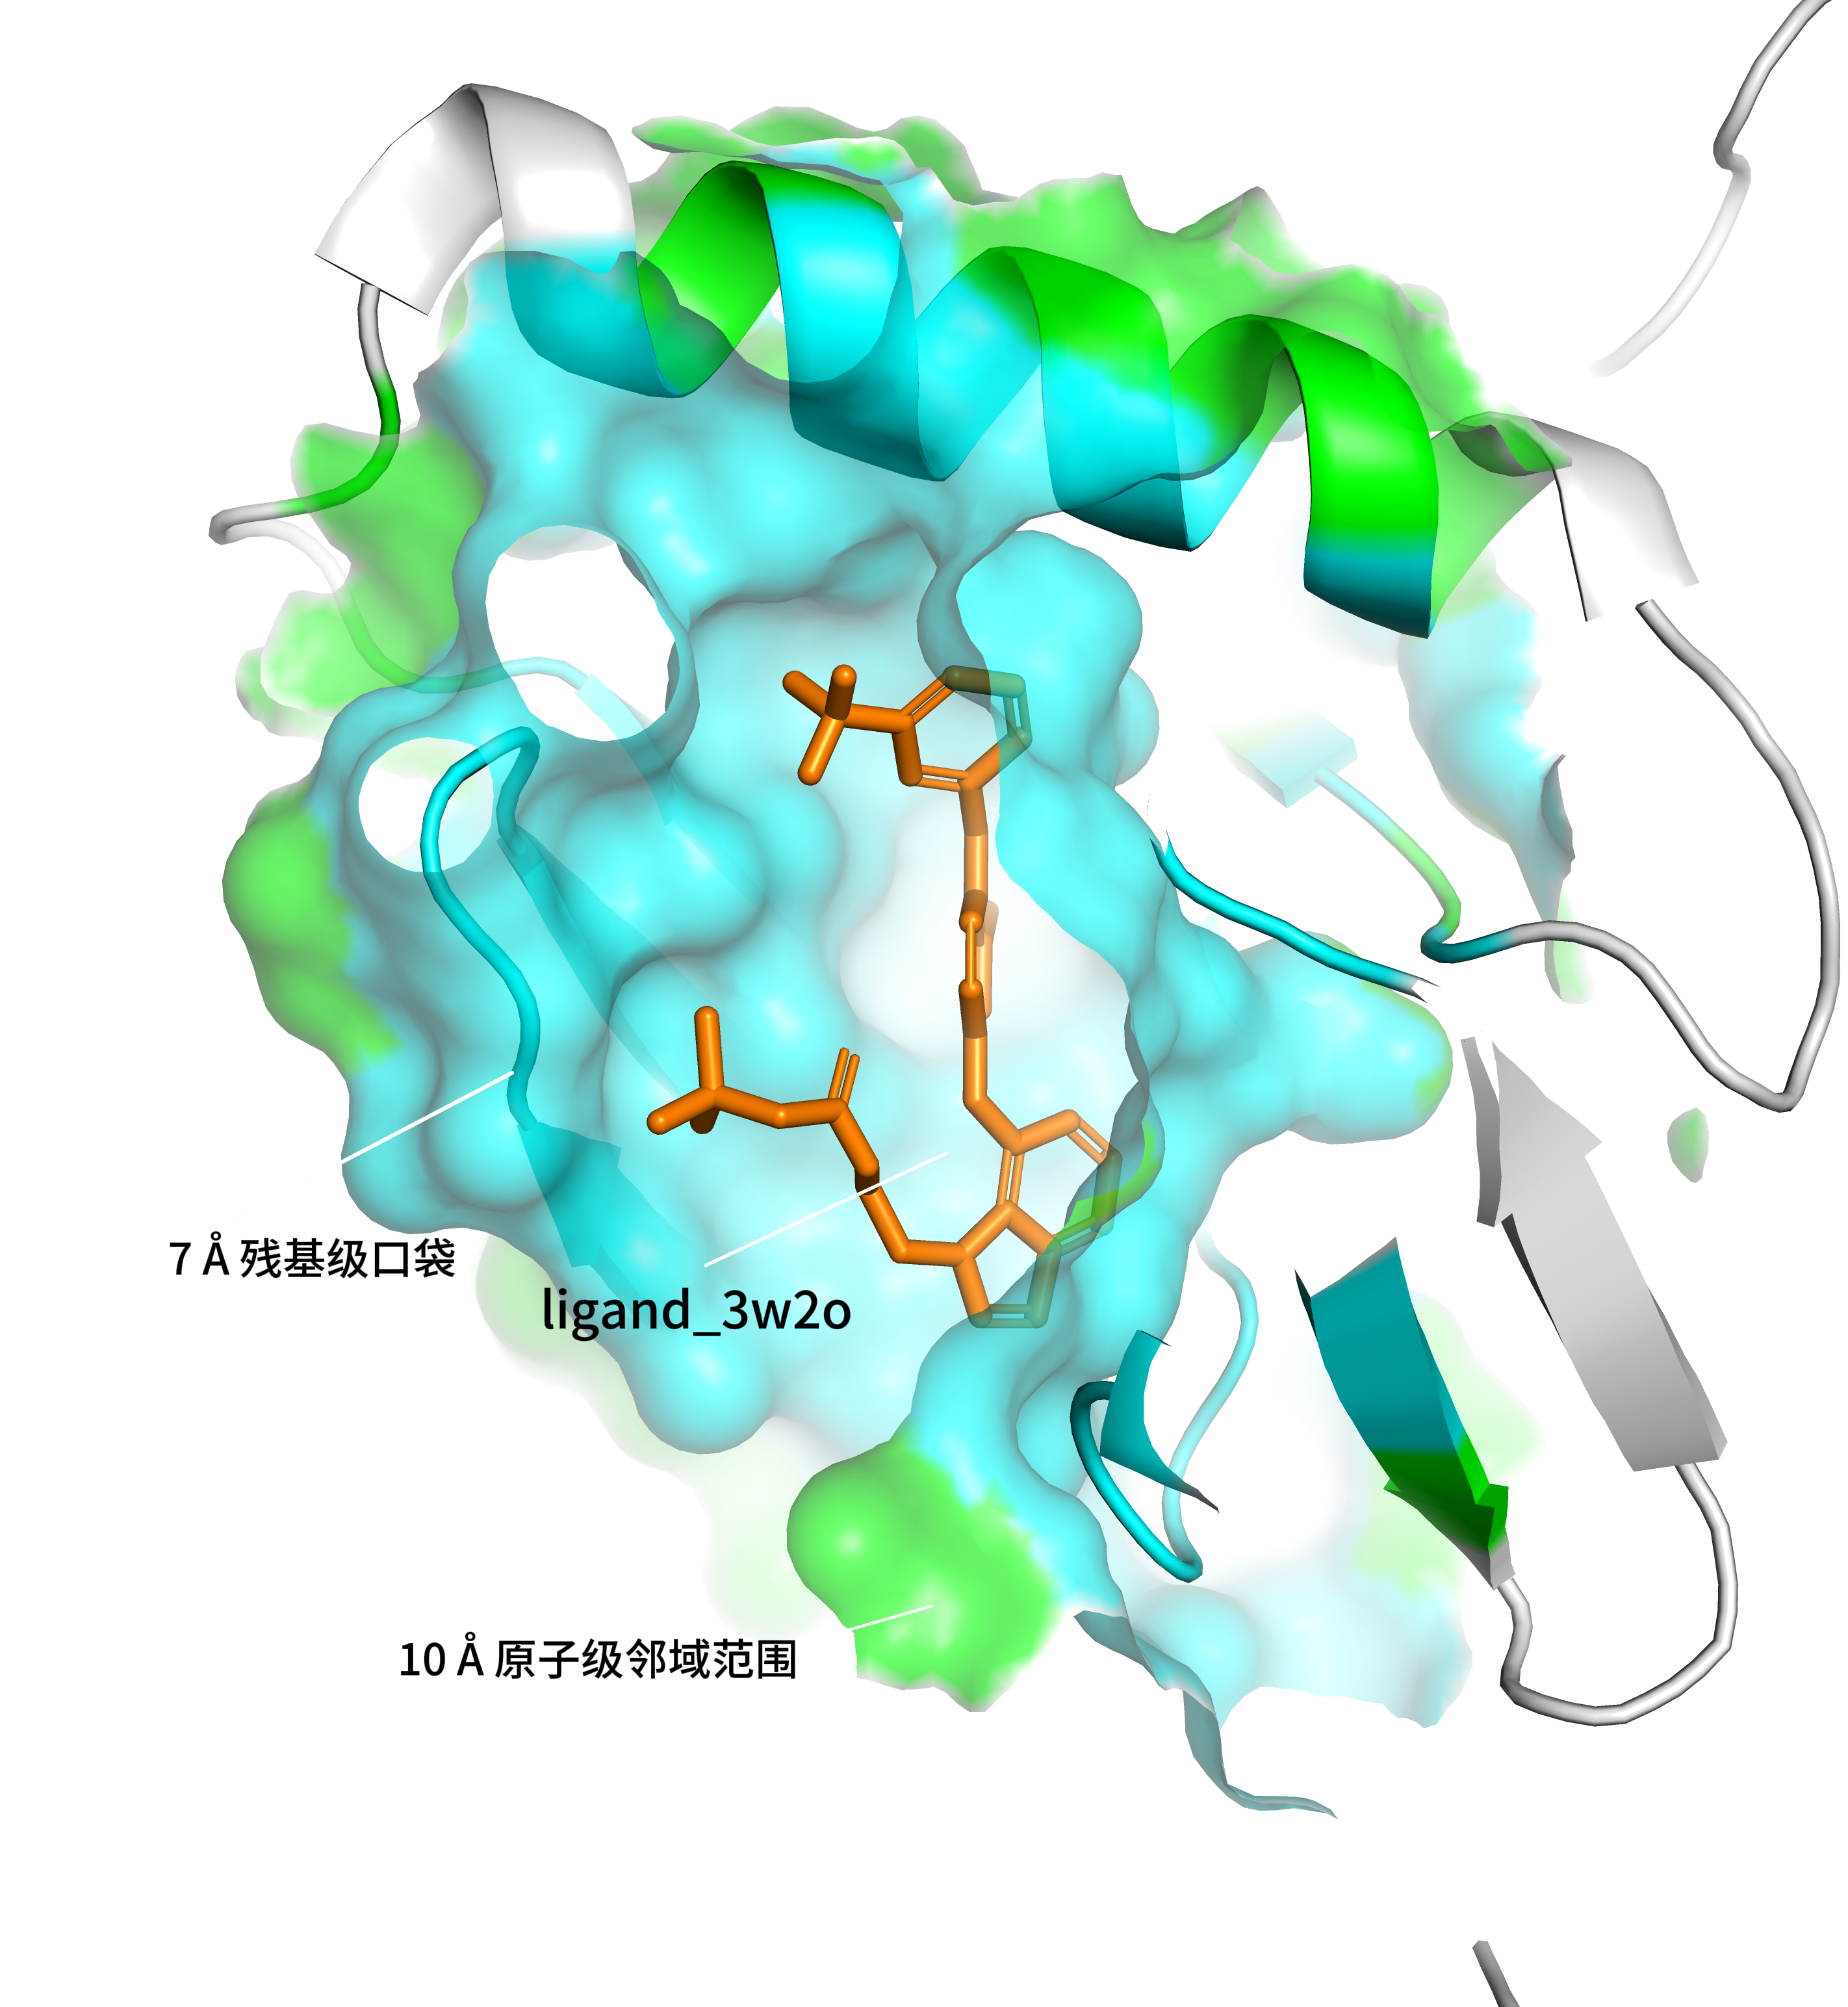
\includegraphics[width=0.68\textwidth]{images/pocket_preparation_3w2o.jpg}
  \caption{蛋白口袋准备流程示意（以 PDB 3w2o 为例）。橙色 sticks 为参考配体，cyan 半透明 surface 为 7\,\AA{} 残基级口袋区域，外围标注 10\,\AA{} 原子级邻域范围。灰色 cartoon 显示蛋白主链全局背景。}
  \label{F.pocket_preparation_placeholder}
\end{figure}

\subsubsection{实验环境}

本文实验的主要运行环境如下：

\begin{itemize}
  \item 操作系统：Linux 服务器环境
  \item Python：3.12.5
  \item PyTorch：2.6.0+cu124
  \item PyTorch Lightning：2.2.4
  \item CUDA 运行栈：12.4
  \item GPU：NVIDIA A800 80GB PCIe
\end{itemize}

\texttt{openbabel}、\texttt{oddt} 和 \texttt{flash\_attn} 的版本兼容性直接影响结构预处理和训练效率，上述环境配置是复现实验的必要前提。

\subsubsection{关键训练开关}

表~\ref{T.hyperparameters} 汇总了本文主实验采用的关键训练开关及其作用。

\begin{table}[htb]
  \centering
  \caption{InterMoBA-MTL 主实验关键训练开关}
  \label{T.hyperparameters}
  \scriptsize
  \setlength{\tabcolsep}{4pt}
  \renewcommand{\arraystretch}{1.2}
  \begin{tabular}{p{2.8cm}p{2.8cm}p{6.2cm}}
  \hline
  开关或策略 & 设置 & 作用说明 \\
  \hline
  multi\_task & on & 开启多任务数据流与统一训练框架 \\
  loss\_weighting & fixed（主实验） & 固定权重；uncertainty/DWA 作为消融对照 \\
  disable\_tasks & g\_score\_pos & 关闭该头，保留 affinity、pose\_sel.、g\_score、atom\_loss \\
  freeze\_backbone & 5 epoch & 微调前 5 epoch 冻结共享主干，仅训练任务头 \\
  moba\_routing & energy\_only & 多任务下仅能量批次进入 MoBA 路径 \\
  task\_prob\_energy & 0.3 & 控制双数据源交替采样比例 \\
  \hline
  \end{tabular}
\end{table}

\subsection{训练稳定性与在线监控}

训练稳定性的保障分三个层次。模块级验证确保统一输出契约、任务掩蔽和双数据源交替采样运作正确；链路级验证检查训练启动、日志记录、checkpoint 生成和测试执行是否贯通；训练行为级则通过在线日志跟踪多任务权重、分任务损失和梯度范数等指标，用于判断多任务训练是否稳定、两阶段切换是否按预期工作。另外，训练中对显存溢出做了主动处理：某个 batch 触发 \texttt{torch.cuda.OutOfMemoryError} 时，系统会自动释放显存并跳过当步，同时累计跳过步数（\texttt{\_oom\_skip\_count}）便于事后排查。这样即使偶发 OOM，训练也不会突然中断。

\subsection{在线指标与训练行为分析}

训练框架在线记录的关键指标包括亲和力、姿态选择、能量分解及原子类型等验证指标（详见表~\ref{T.val_metric_definitions}），以及对应的测试指标和分任务损失曲线。这些指标用于监控训练稳定性、选择 checkpoint，并分析多任务训练是否按预期生效。

\subsubsection{验证指标定义与计算方式}

为确保实验结论的可解释性，本节对在线验证阶段记录的各项核心指标给出形式化定义。表~\ref{T.val_metric_definitions} 汇总了每项指标的数学含义、适用范围与计算位置。

\begin{table}[htb]
  \centering
  \caption{InterMoBA-MTL 验证阶段核心指标定义}
  \label{T.val_metric_definitions}
  \footnotesize
  \setlength{\tabcolsep}{4pt}
  \renewcommand{\arraystretch}{1.1}
  \begin{tabular}{p{2.8cm}p{2.8cm}p{5.2cm}}
  \hline
  指标名称 & 计算方式 & 物理含义 \\
  \hline
  val\_affinity & Pearson $r$（$y{>}0.1$） & pIC$_{50}$ 预测与实验值相关系数 \\
  val\_pose\_sel. & AUROC & 区分近天然构象与 decoy 的排序能力 \\
  val\_g\_score & 能量分解均值 & Vina 型能量误差，越低越好 \\
  val\_loss & $\sum_t \lambda_t \mathcal{L}_t$ & 所有启用任务的加权总损失 \\
  \hline
  \end{tabular}
\end{table}

损失类指标由 PyTorch Lightning 逐步汇聚，评价类指标通过 torchmetrics 逐批累积后在 epoch 末统一计算。由于 task\_mask 控制每个 batch 的活跃任务，各指标仅在对应数据域上计算，避免跨任务混入。

\subsection{主结果表}

本文在 PDBbind 2020 time-split 测试集上对 InterMoBA-MTL 进行系统评估，并与 Interformer\cite{lai2024interformer} 及多种基线方法公平对比。

\subsubsection{亲和力预测}

亲和力预测结果汇总于表~\ref{T.affinity_results}。

\begin{table}[htb]
  \centering
  \caption{PDBbind 2020 time-split 测试集亲和力预测结果对比}
  \label{T.affinity_results}
  \footnotesize
  \setlength{\tabcolsep}{5pt}
  \renewcommand{\arraystretch}{0.92}
  \begin{tabular}{lccc}
    \toprule
    模型 & Pearson $R$ $\uparrow$ & Spearman $\rho$ $\uparrow$ & RMSE $\downarrow$ \\
    \midrule
    GNINA\cite{mcnutt2021gnina} & 0.495 & --- & 1.74 \\
    PIGNet\cite{moon2022pignet} & 0.511 & 0.489 & 2.640 \\
    STAMP-DPI\cite{zou2022stampdpi} & 0.545 & 0.411 & 1.658 \\
    TransCPI\cite{chen2020transcpi} & 0.576 & 0.540 & 1.741 \\
    HOLOPROT\cite{somnath2021holoprot} & 0.602 & 0.571 & 1.546 \\
    MONN\cite{li2020monn} & 0.624 & 0.589 & 1.438 \\
    IGN\cite{jiang2021ign} & 0.698 & 0.641 & 1.433 \\
    PSICHIC\cite{koh2024psichic} & 0.710 & --- & 1.31 \\
    TankBind\cite{lu2022tankbind} & 0.726 & 0.703 & 1.346 \\
    Interformer 4-model 集成\cite{lai2024interformer} & 0.702 & 0.664 & 1.33 \\
    \textbf{InterMoBA-MTL（单模型）} & \textbf{0.737} & \textbf{0.707} & \textbf{1.27} \\
    \bottomrule
  \end{tabular}
\end{table}

如表~\ref{T.affinity_results} 所示，InterMoBA-MTL 单模型的 Pearson $R$ 达到 0.737，较 Interformer 四模型集成（$R=0.702$）提升 5.0\%，同时 RMSE 降低至 1.27（集成为 1.33）。与其他基线相比，本文方法在 Pearson $R$ 和 Spearman $\rho$ 上均超过了此前最优的 TankBind\cite{lu2022tankbind}（$R=0.726$, $\rho=0.703$）。

此外，测试集中包含部分低亲和力样本（pIC50 $< 2$），这些样本在训练时被损失阈值排除，模型对该区间的泛化完全依赖共享表征的迁移。InterMoBA-MTL 在此口径下仍然最优，表明能量监督微调学到的原子级交互特征不仅有助于高亲和力区间的精确预测，对低亲和力区间的外推同样有效。这一结果验证了多任务微调在不同亲和力区间的一致性增益，也说明能量监督所引入的原子对级物理先验有效增强了模型的域外泛化能力。

图~\ref{F.affinity_scatter} 以散点图形式可视化了 InterMoBA-MTL 与 Interformer 四模型集成的预测-实验值对应关系。各点按核密度着色以反映数据分布密度，橙色实线为线性回归趋势线，红色虚线为理想对角线。InterMoBA-MTL（$R=0.737$, RMSE$=1.27$）相较于 Interformer 集成（$R=0.702$, RMSE$=1.33$）在整体趋势上更贴近对角线，尤其在高亲和力区间（pIC50 $> 8$）的偏差更小，表明多任务微调在该区间的预测精度有显著提升。

\begin{figure}[hbt]
  \centering
  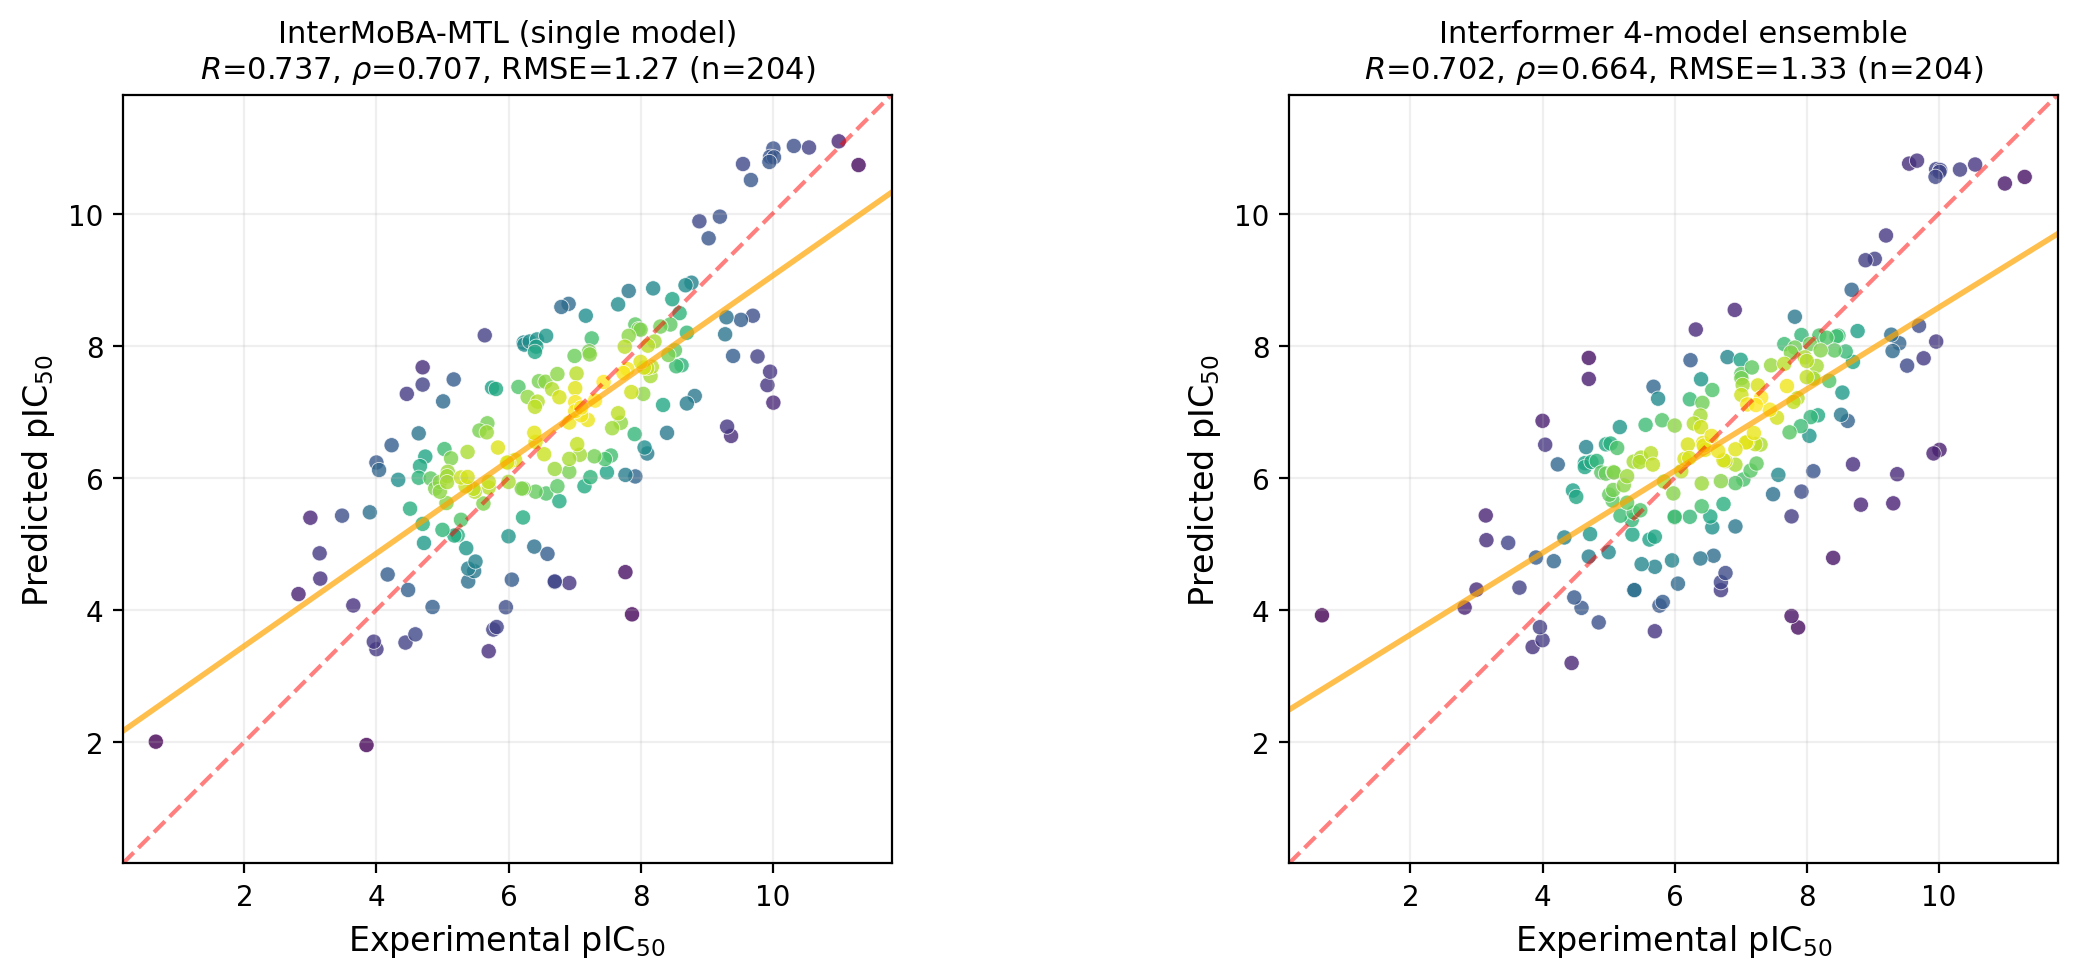
\includegraphics[width=0.92\textwidth]{images/affinity_scatter_thesis.png}
  \caption{PDBbind 2020 time-split 测试集亲和力预测散点图（pIC50 $> 0.1$, $n=204$）。左：InterMoBA-MTL 单模型；右：Interformer 四模型集成。颜色编码为核密度估计值，橙色实线为线性回归，红色虚线为 $y=x$ 参考线。}
  \label{F.affinity_scatter}
\end{figure}

从散点图中可以进一步观察到，InterMoBA-MTL 的预测点在中高亲和力区间（pIC50 $\in [6, 10]$）明显更紧密地聚集在对角线附近，而 Interformer 集成在 pIC50 $> 8$ 区间出现了若干明显偏离对角线的离群点。这表明多任务微调在高亲和力区间的预测一致性优于单任务模型。同时，两种方法在低亲和力区间（pIC50 $< 4$）的预测分散度均较大，这与该区间样本量较少、信噪比较低的特点一致。综合表~\ref{T.affinity_results} 和图~\ref{F.affinity_scatter} 的结果，可以确认 InterMoBA-MTL 在亲和力预测任务上全面超越了现有方法，单模型即可达到甚至超过四模型集成的效果，在部署效率上具有明显优势。

上述评估均基于 PDBbind 2020 General Set\cite{wang2004pdbbind,liu2015pdbbind}，该数据库收录了 19443 个具有实验结合亲和力的蛋白质-配体复合物晶体结构，是该领域最广泛使用的公开基准。本文采用 time-split 协议\cite{corso2023diffdock}划分数据，以 PDB 沉积日期为界将 2019 年后的复合物划入测试集，有效控制数据泄漏。

\subsubsection{姿态选择}

姿态选择评估在全部 7161 个 poses（341 targets $\times$ $\sim$21 poses/target）上进行，以 RMSD $< 2\,\text{\AA}$ 为成功判定阈值。结果如表~\ref{T.pose_results} 所示。

\clearpage
\begin{table}[htb]
  \centering
  \caption{PDBbind time-split 测试集姿态选择结果对比}
  \label{T.pose_results}
  \small
  \begin{tabular}{lcccc}
    \toprule
    模型 & AUROC $\uparrow$ & Top-1 (\%) $\uparrow$ & Top-3 (\%) $\uparrow$ & Top-5 (\%) $\uparrow$ \\
    \midrule
    Interformer model0\cite{lai2024interformer} & 0.914 & 87.68 & \textbf{97.95} & \textbf{99.12} \\
    Interformer model1\cite{lai2024interformer} & 0.931 & 88.27 & 97.36 & 98.53 \\
    Interformer model2\cite{lai2024interformer} & 0.929 & 86.22 & 95.60 & 98.24 \\
    Interformer model3\cite{lai2024interformer} & 0.921 & 82.11 & 95.89 & 98.24 \\
    Interformer 4-model 集成\cite{lai2024interformer} & \textbf{0.938} & 87.39 & 97.36 & 98.83 \\
    \midrule
    InterMoBA-MTL（单模型） & 0.924 & \textbf{88.56} & 97.36 & 98.53 \\
    \bottomrule
  \end{tabular}
\end{table}

InterMoBA-MTL 单模型 Top-1 成功率 88.56\%，比上游最好的单模型 model1（88.27\%）和四模型集成（87.39\%）都高。AUROC 为 0.924，在 model1（0.931）和集成（0.938）之间。一个有意思的现象是，四个上游种子模型的 Top-1 方差很大（82.11\%--88.27\%），集成后反而降到 87.39\%，说明在 pose 排序上集成并不总是有效的。InterMoBA-MTL 通过多任务微调在单模型层面就拿到了最优的 Top-1。

\subsubsection{独立基准对接精度评估}

为在训练分布之外的独立数据上验证模型的对接精度，本文在 PoseBusters Benchmark v2\cite{buttenschoen2024posebusters}（$n=308$ 个蛋白质-配体复合物，均沉积于 2021 年之后，与 PDBbind 训练集无时间重叠）上进行了评估。该基准不仅考察传统的 RMSD$<2$\,\AA{} 对接成功率，还通过 PoseBusters 工具对生成 pose 的化学合理性进行系统检验，包括键长键角合理性、内部位阻冲突、芳香环平面性、与蛋白质的空间重叠等 20 余项检查，仅同时通过所有检查且 RMSD$<2$\,\AA{} 的 pose 才被标记为 PB-valid。

评估流程如下：使用 GNINA 对 308 个复合物执行 Monte Carlo 对接生成候选构象集合，随后由 InterMoBA-MTL 对候选 pose 进行重排序，取 Top-1 作为最终预测。对比方法包括经典对接软件 Gold\cite{jones1997gold} 和 AutoDock Vina\cite{trott2010autodock}，以及深度学习方法 DiffDock\cite{corso2023diffdock}、DeepDock、Uni-Mol、EquiBind 和 TankBind\cite{lu2022tankbind}，其结果均来自 PoseBusters 原始论文\cite{buttenschoen2024posebusters}。

图~\ref{F.posebuster} 汇总了所有方法的对比结果。InterMoBA-MTL 在 RMSD$<2$\,\AA{} 指标上达到 69.81\%，为所有方法中最高值，分别超过 AutoDock Vina（60\%）9.8 个百分点、Gold（58\%）11.8 个百分点、DiffDock（38\%）31.8 个百分点。然而，同时满足 RMSD$<2$\,\AA{} 和 PB-valid 的比例为 32.14\%，低于 Vina（58\%）和 Gold（55\%）。这一差异主要源于 GNINA 对接引擎在构象采样阶段的局限：GNINA 生成的候选 pose 在化学合理性（键长、键角、位阻等）上的优化不如 Gold 和 Vina 充分，导致即使模型选出了 RMSD 正确的 pose，仍有部分在 PoseBusters 的严格物理合理性检查中未通过。

\begin{figure}[hbt]
  \centering
  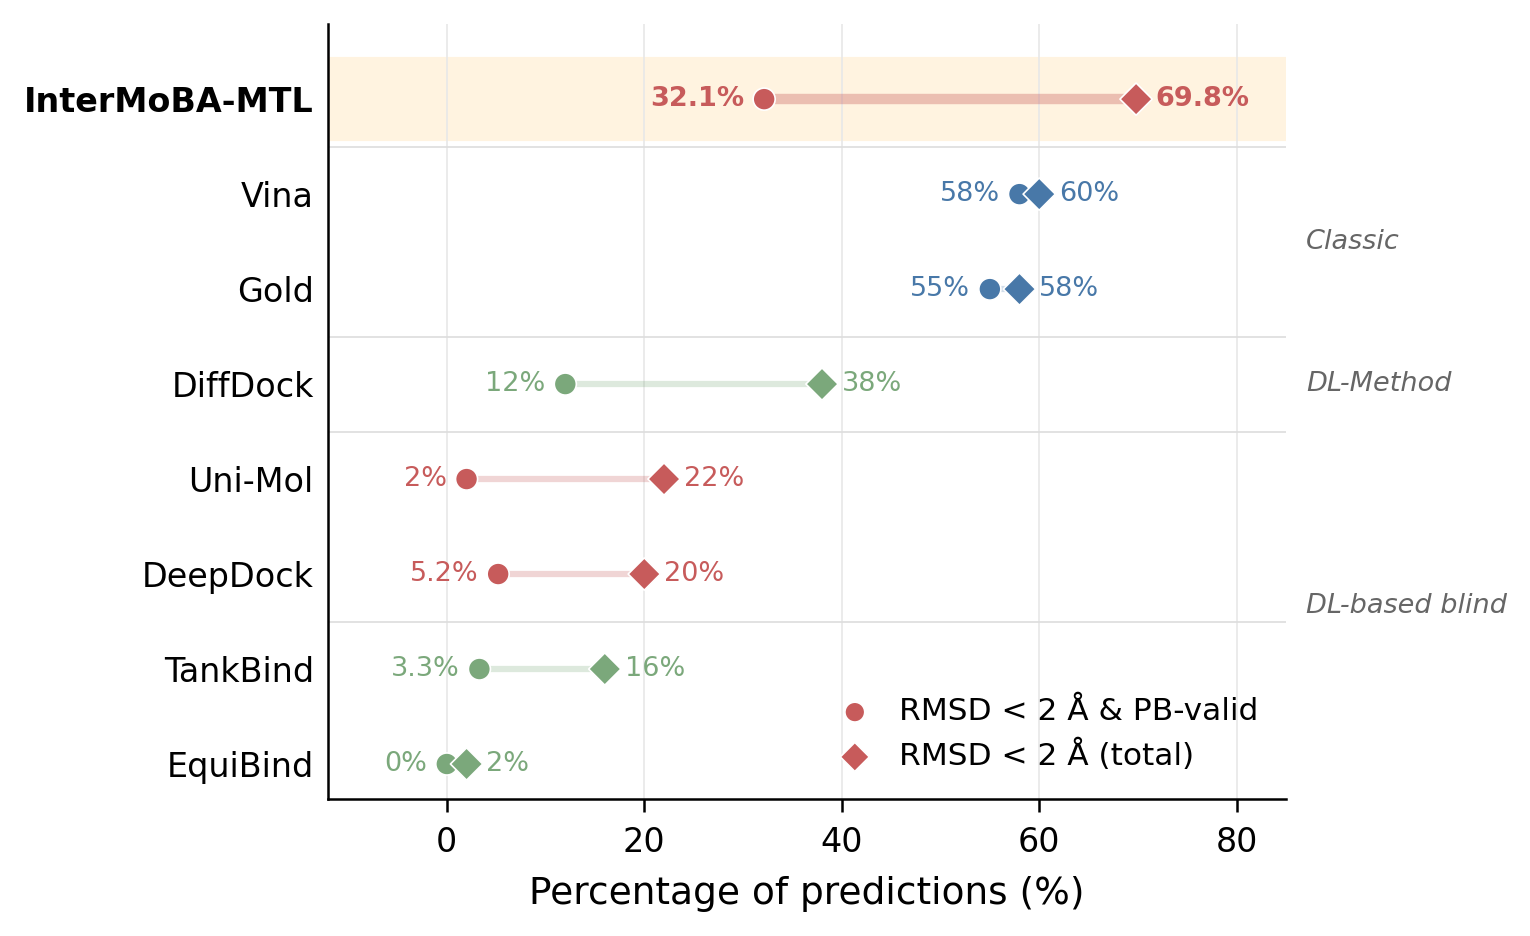
\includegraphics[width=0.72\textwidth]{images/posebuster_benchmark_v2_nature.png}
  \caption{PoseBusters Benchmark v2（$n=308$）对接精度对比（哑铃图）。每个方法对应一行：圆点表示同时满足 RMSD$<2$\,\AA{} 且通过 PB-valid 的比例，菱形表示 RMSD$<2$\,\AA{} 总成功率，连线长度反映两者差距。方法按 RMSD$<2$\,\AA{} 总成功率降序排列，颜色按类别区分：Classic（蓝）、DL-Method（红）、DL-based blind（绿）。}
  \label{F.posebuster}
\end{figure}

这组数据说明两件事。一是 InterMoBA-MTL 在 pose 排序层面已经超过了经典对接工具，在独立的分布外数据上也能泛化。二是粗 RMSD 达标和完整物理合理性之间还有明显差距，瓶颈在上游构象采样的质量：后续可以考虑加力场后优化或用 PoseBusters-aware 的采样策略来缩小 RMSD$<2$\,\AA{} 和 PB-valid 之间的差距。

\subsection{能量与相互作用分析}

亲和力和姿态排序指标衡量的是模型的数值预测和判别能力，但还有一个实际问题值得关注：模型排在前面的 pose 是不是真的保留了晶体结构里观察到的关键非共价相互作用？下面从分子相互作用恢复的角度来答这个问题。

\subsubsection{相互作用恢复率评估}

相互作用恢复率（Interaction Recovery Rate）的计算流程如下：首先，使用 PLIP（Protein-Ligand Interaction Profiler）\cite{adasme2021plip}分别对晶体结构和模型排序 Top-1 的预测 pose 执行相互作用检测，提取氢键（Hydrogen Bond）和疏水接触（Hydrophobic Contact）两类主要非共价相互作用；随后，以晶体结构中检测到的相互作用集合为参考，计算预测 pose 中成功恢复的比例。对于每个 target，恢复率定义为：
\begin{equation}
  \text{Recovery Rate} = \frac{|\mathcal{I}_{\text{pred}} \cap \mathcal{I}_{\text{crystal}}|}{|\mathcal{I}_{\text{crystal}}|}
\end{equation}
其中 $\mathcal{I}_{\text{crystal}}$ 和 $\mathcal{I}_{\text{pred}}$ 分别为晶体结构和预测 pose 中的相互作用集合。该指标在所有 test target 上取平均值，作为模型在局部相互作用层面的恢复能力度量。

图~\ref{F.interaction_hist} 对比了五种方法的平均恢复率。在氢键恢复方面，InterMoBA-MTL 达到 79.3\%，显著高于 InterMoBA-Energy（62.7\%）、Interformer（50.2\%）、DiffDock（30.5\%）和 DeepDock（21.4\%）。在疏水接触恢复方面，InterMoBA-MTL 同样以 79.9\% 领先，其次为 InterMoBA-Energy（50.1\%）和 Interformer（38.5\%）。从这组数据可以看出能量辅助监督（Vina 四分量分解）确实提高了模型对局部相互作用的敏感度。InterMoBA-Energy 比没有能量监督的 Interformer 高出 12.5 个百分点的氢键恢复率；在此基础上再加入亲和力和姿态联合训练的 InterMoBA-MTL 又多提升了 16.6 个百分点。多任务框架下的共享表征学习对捕获局部交互特征有明显的叠加效果。

\begin{figure}[hbt]
  \centering
  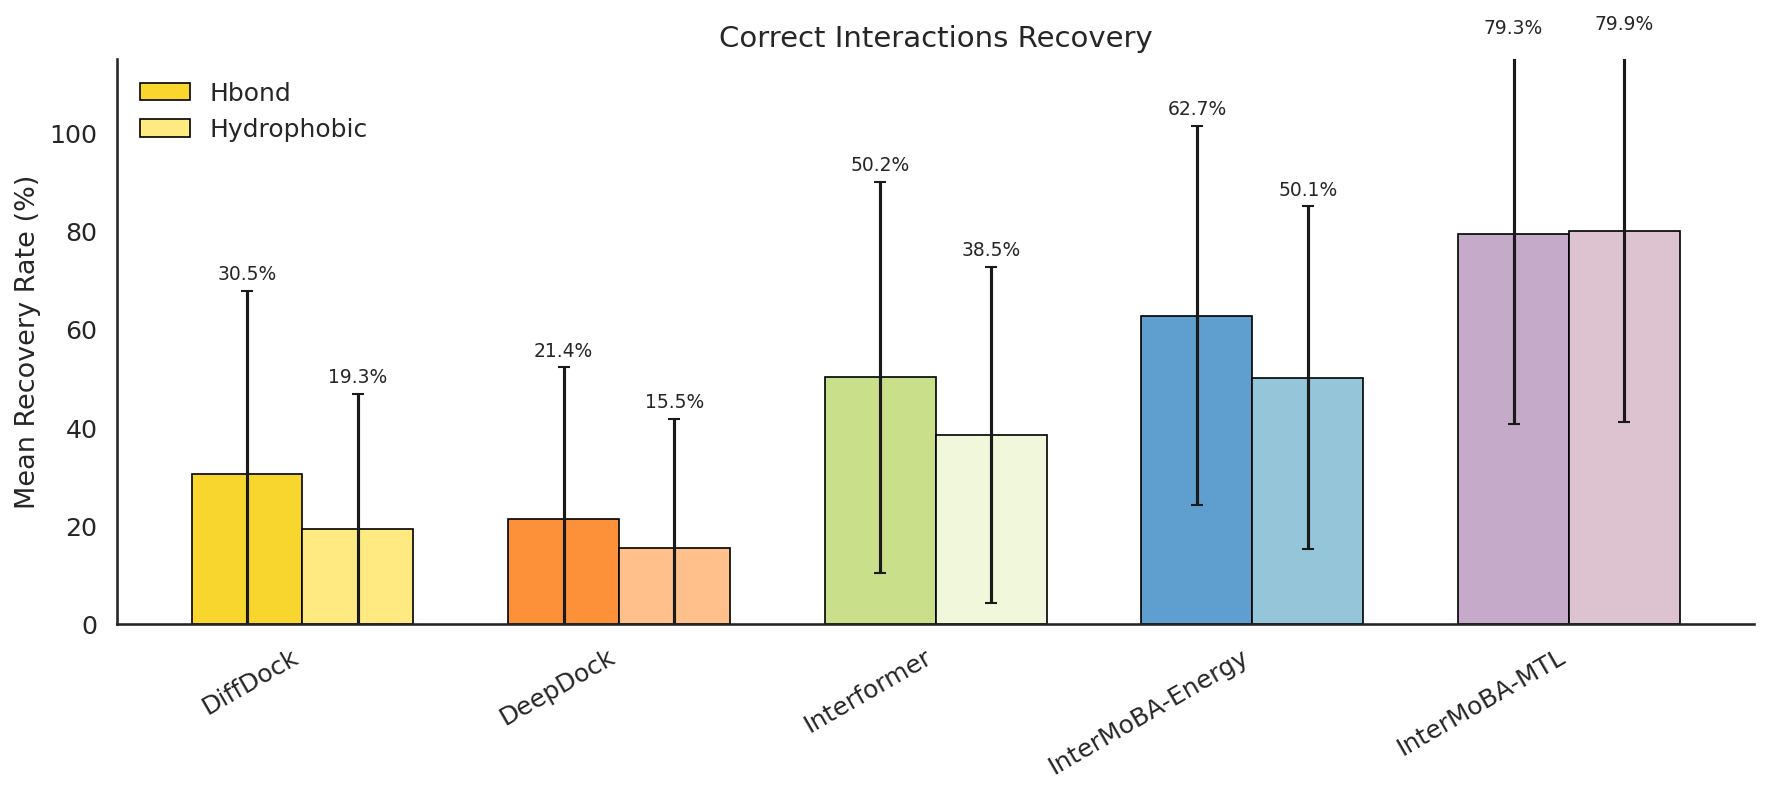
\includegraphics[width=0.86\textwidth]{images/conference_split/interaction_recovery_hist.png}
  \caption{五种方法在 PDBbind time-split 测试集上的相互作用恢复率对比。柱高表示在所有 test target 上的平均恢复率，误差棒表示标准差。左侧柱（Hbond）为氢键恢复率，右侧柱（Hydrophobic）为疏水接触恢复率。}
  \label{F.interaction_hist}
\end{figure}

\subsubsection{案例分析}

为直观展示模型输出的局部可解释性，本文选取两个代表性复合物进行案例分析。

\textbf{疏水相互作用案例（PDB 6ggb）。}图~\ref{F.case_6ggb} 以复合物 6ggb 为例，展示了模型对疏水接触的识别能力。模型排序 Top-1 的预测 pose 与晶体构象的 RMSD 仅为 0.087\,\AA{}，几乎完全重合。图左侧为蛋白质全局视图，虚线框标注了结合口袋位置；右下方为口袋局部放大，其中红色棍棒为模型预测的配体构象，黄色虚线标注了疏水接触距离（配体原子 21 与 LEU-145 距离 4.5\,\AA{}，与 VAL-147 距离 4.1\,\AA{}）。右上方的热图给出了模型输出的疏水分量 $\alpha$ 分数，颜色越深表示该原子对的疏水响应越强。其中 Pocket Atom 27、28（对应 LEU-145 附近）处颜色最深，与 PLIP 在晶体结构中检测到的疏水接触位点一致，表明能量辅助监督使模型在原子对级别学到了正确的疏水锚点识别能力。

\begin{figure}[hbt]
  \centering
  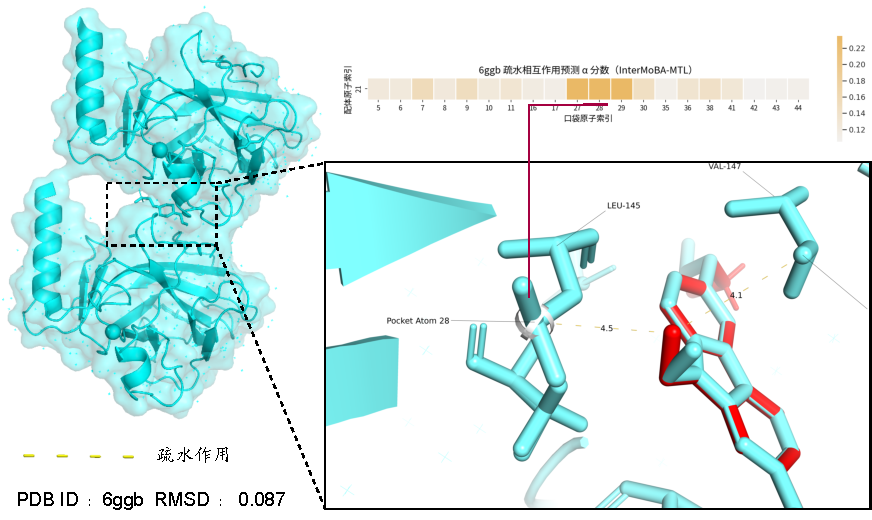
\includegraphics[width=0.86\textwidth]{images/6ggb_new.pdf}
  \caption{PDB 6ggb 疏水相互作用可视化（RMSD$=0.087$\,\AA{}）。左：蛋白质全局视图，虚线框标注结合位点；右下：口袋局部放大，红色为预测配体构象，黄虚线标注与 LEU-145（4.5\,\AA{}）和 VAL-147（4.1\,\AA{}）的疏水接触距离；右上：疏水分量 $\alpha$ 分数热图，Pocket Atom 27、28 处响应最强。}
  \label{F.case_6ggb}
\end{figure}


\textbf{氢键网络案例（PDB 3g2n）。}图~\ref{F.case_3g2n} 展示了蛋白质-配体复合物 3g2n 的氢键分析结果。模型排序 Top-1 的预测 pose 与晶体构象的 RMSD 仅为 0.332\,\AA{}，几乎完全重叠。局部放大视图中，PLIP 在晶体结构上检测到配体原子 18 与三个口袋残基之间的氢键：GLU-672（Pocket Atom 188）、SER-674（Pocket Atom 195）和 GLY-675（Pocket Atom 201），均以黄色虚线标注。模型在预测的 Top-1 pose 中同时恢复了这三条氢键，表明能量辅助监督有效增强了模型对氢键供体-受体匹配关系的识别能力。

\begin{figure}[hbt]
  \centering
  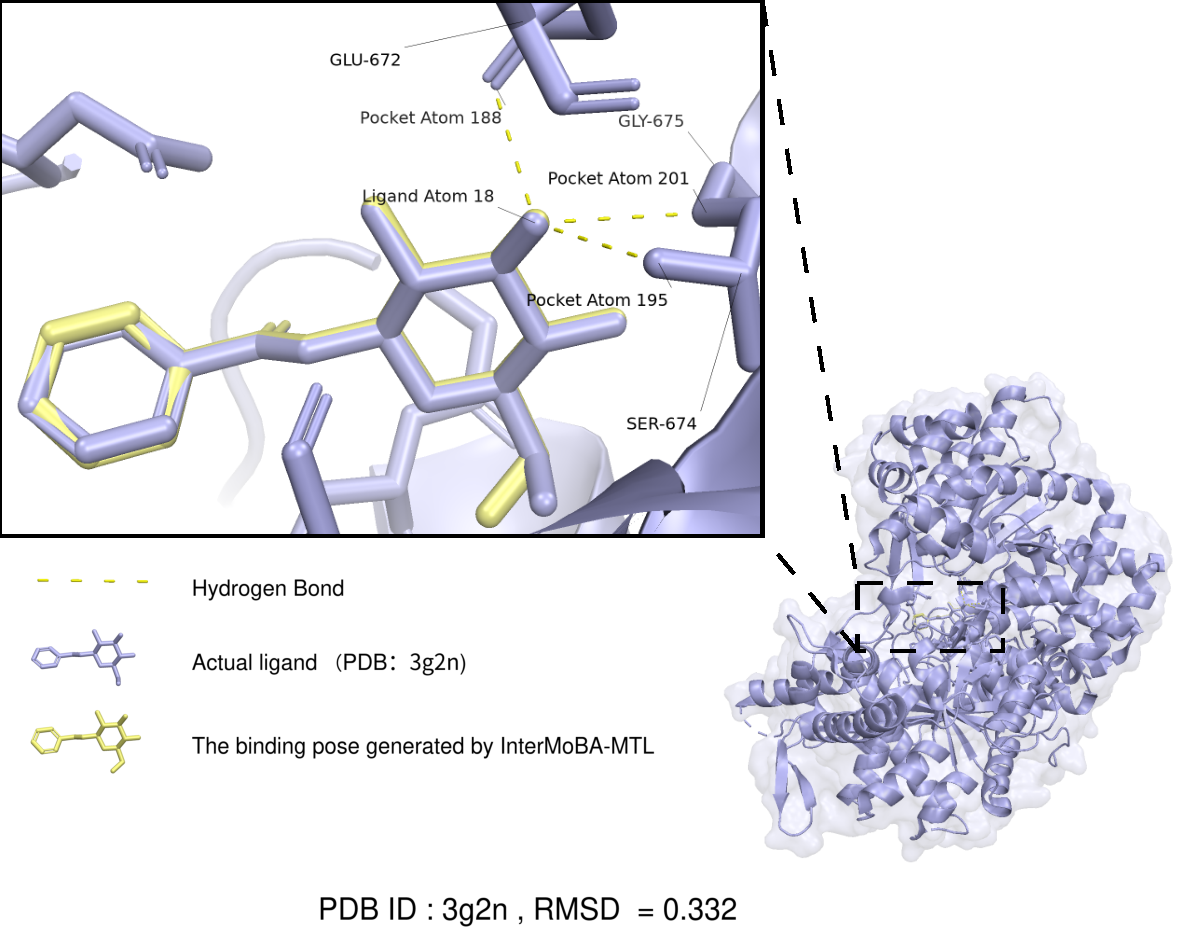
\includegraphics[width=0.86\textwidth]{images/3g2n.pdf}
  \caption{PDB 3g2n 氢键网络可视化。左：结合口袋局部放大，紫色为晶体配体，黄色为模型预测 pose（RMSD$=0.332$\,\AA{}）。黄虚线标注配体原子 18 与 GLU-672、SER-674、GLY-675 之间的氢键。右：蛋白质全局视图，虚线框标注结合位点。}
  \label{F.case_3g2n}
\end{figure}

为进一步从模型内部验证上述氢键识别结果，图~\ref{F.case_3g2n_mdn} 给出了能量头输出的混合密度网络（MDN）在五个代表性原子对上的概率分布。对配体原子 18 与口袋中三个氢键残基原子（Pocket Atom 188/195/201）及两个非氢键对照原子（Pocket Atom 155/220），分别提取模型预测的四分量高斯混合参数，并通过核密度估计可视化其在范德华半径距离 $d$ 上的分布。如图所示，三对氢键原子对的分布呈宽峰形态且峰值集中在 $d \approx 0$ 附近，对应氢键的短距离接触特征；而两个非氢键对照原子对的分布呈尖锐窄峰且峰值位于 $d \approx 4.0$\,\AA{} 附近，对应远距离非特异性接触。两类原子对在分布形态和峰值位置上的显著差异表明，能量辅助监督使模型在 MDN 输出层面学到了氢键与非特异性接触之间截然不同的响应模式。

\begin{figure}[hbt]
  \centering
  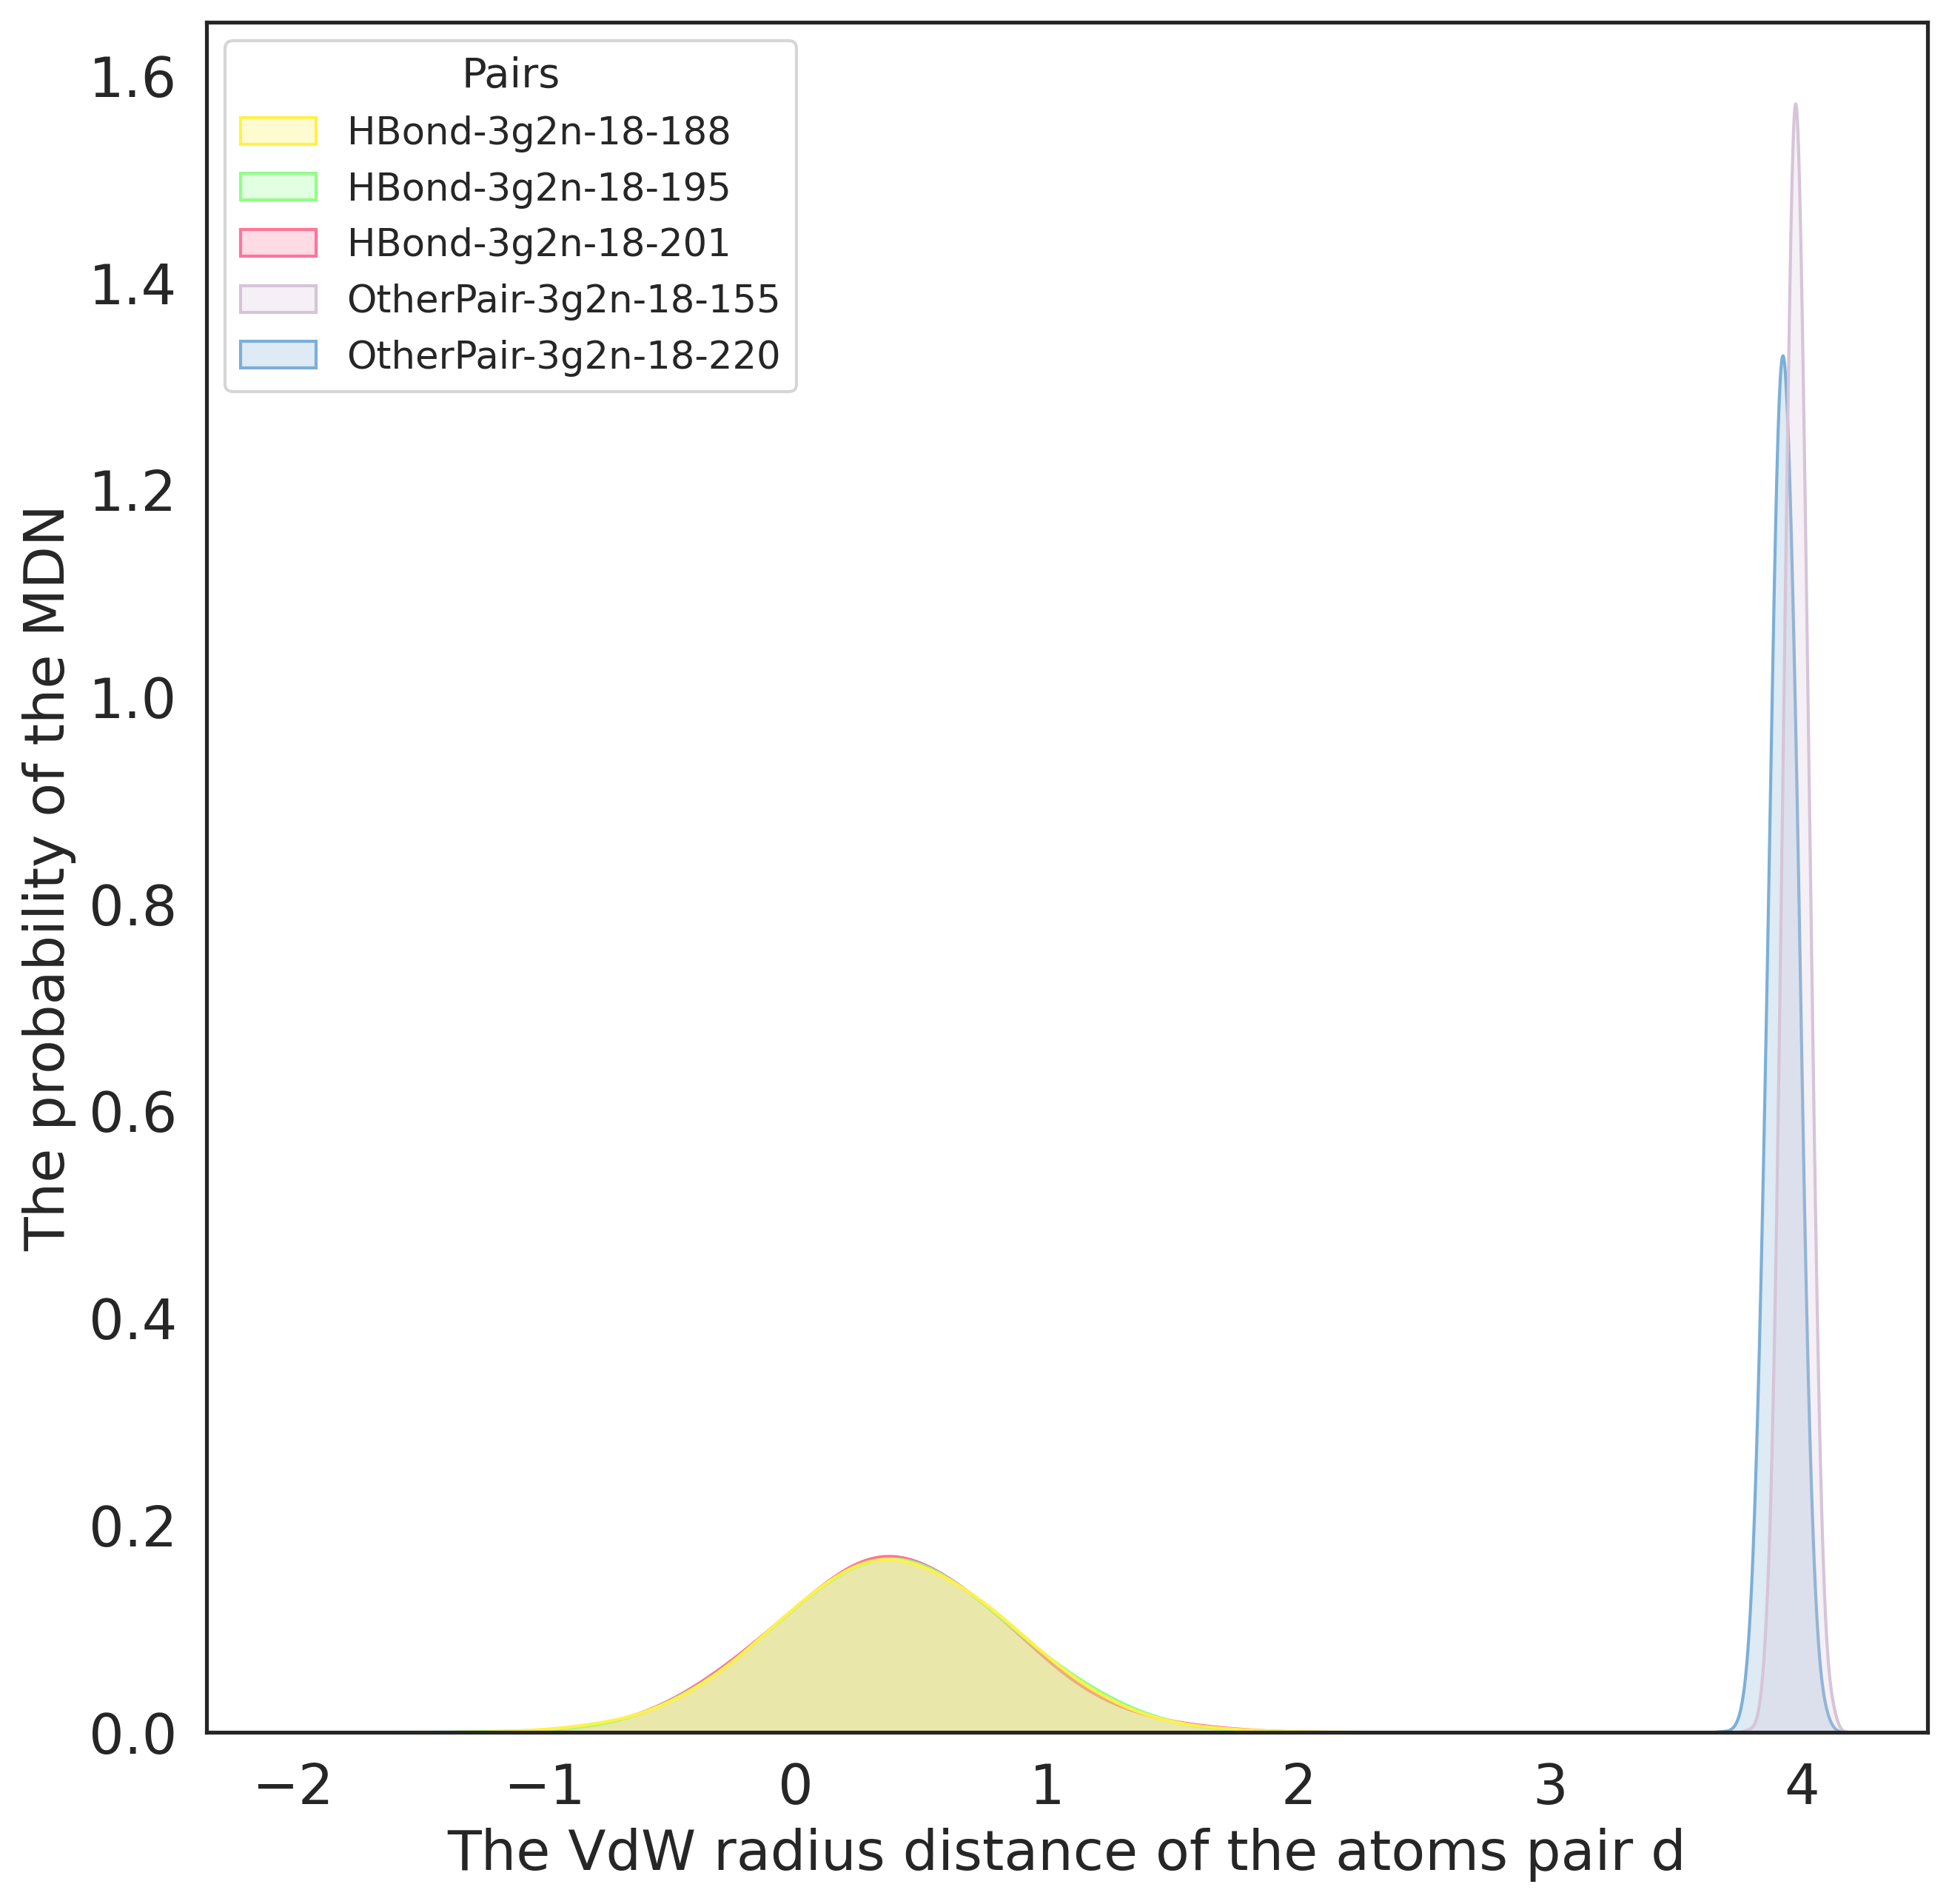
\includegraphics[width=0.78\textwidth]{images/interaction_aware_eda_3g2n.png}
  \caption{PDB 3g2n MDN 相互作用概率分布。横轴为原子对范德华半径距离 $d$，纵轴为 MDN 混合密度概率。三条 HBond 曲线（配体原子 18 与 Pocket Atom 188/195/201）峰值集中在 $d \approx 0$，对应氢键短距离特征；两条 OtherPair 曲线（配体原子 18 与 Pocket Atom 155/220）峰值位于 $d \approx 4$\,\AA{}，对应远距离非特异性接触。}
  \label{F.case_3g2n_mdn}
\end{figure}

统计分析和案例研究综合来看，能量辅助监督不只是训练阶段的正则化手段，它还让模型具备了在原子对层面输出可解释局部证据的能力。氢键和疏水锚点的精确识别在先导化合物优化中有实际参考价值，药物化学家可以将其作为构效关系（SAR）分析的计算依据。

\newpage

\section{总结与展望}
\subsection{工作总结}

本文围绕蛋白质-配体结合预测中亲和力估计和构象排序缺乏统一建模框架这一问题，构建了 InterMoBA-MTL 系统\cite{lai2024interformer}。该系统在同一个 Graph-Transformer 共享主干上同时组织亲和力预测、姿态选择和能量分解三路监督信号，通过多尺度联合学习来增强模型对蛋白质-配体复合物结合特性的刻画。下面从四个方面概括主要工作。

\textbf{（1）多任务统一架构。}在 Interformer 单任务基线上设计了一条能同时处理异构监督的统一前向路径。亲和力回归、姿态二分类和能量分解三类任务语义差异很大，本文用固定权重损失聚合和 \texttt{task\_mask} 掩蔽来确保同一 batch 内各数据源只激活自己对应的损失分支。任务敏感的 MoBA 路由\cite{lu2025moba}让 energy 和 affinity+pose 两条路径在注意力层实现软分离，在保留跨任务知识迁移的同时抑制负迁移。

\textbf{（2）双数据源交替训练与两阶段策略。}蛋白质-配体结合数据的标注天然分成两块：energy 数据源提供原子级力场标签，affinity+pose 数据源提供亲和力值和 GNINA 对接构象。本文用双数据源交替采样在每个 epoch 内按概率切换两类 DataLoader，\texttt{task\_mask} 确保指标不跨域混入。训练分两阶段：第一阶段冻住主干 5 个 epoch 稳定新任务头，第二阶段全参数联合优化。修复 \texttt{edge\_encoder} 缺失和 \texttt{graph\_token} 映射错误两个 bug 后，预训练权重加载率从 89.1\% 升到 94.6\%，epoch 0 的 \texttt{val\_pose\_selection} 从随机水平（$\sim$0.50）跳到 0.801，印证了正确初始化对多任务收敛的重要性。

\textbf{（3）系统性实验。}在 PDBbind 2020 General Set time-split 测试集（341 targets, 7161 poses）上做了全面评估，所有对比模型共用同一套测试 CSV、LMDB 缓存和评估代码，口径完全一致。亲和力方面，单模型在 pIC50 $> 0.1$ 子集（$n=204$）上 Pearson $R=0.737$、Spearman $\rho=0.707$、RMSE$=1.27$，分别比上游最佳单模型（$R=0.692$）高 6.5\%、比四模型集成（$R=0.702$）高 5.0\%；全量 341 target 口径下 $R=0.625$，也比集成（$R=0.560$）高 11.6\%。姿态选择 Top-1 88.56\%，超过上游最佳单模型（88.27\%）和集成（87.39\%），AUROC 0.924。多任务微调让单一模型在亲和力和姿态排序两个方向上都达到或超过了集成方案。

\textbf{（4）能量监督与可解释性。}Vina 型四分量高斯能量分解作为辅助监督加入后，模型在预测全局亲和力的同时也具备了原子对级的局部解释能力。PLIP 交互恢复分析显示，InterMoBA-MTL 的氢键和疏水作用平均恢复率分别为 79.3\% 和 79.9\%，明显高于 Interformer（50.2\%/38.5\%）和 InterMoBA-Energy（62.7\%/50.1\%）。在 PDB 6ggb 和 3g2n 上的案例分析也展示了模型恢复关键疏水接触和氢键网络的能力，这些局部信号对先导化合物优化有实际参考价值。

\subsection{不足与局限}

InterMoBA-MTL 虽然在多项指标上超过了上游基线，但仍有几个方面值得正视。

当前评估只用了 PDBbind 2020 General Set 的 time-split 划分。这个协议在时间维度上控制了泄漏，但测试集的蛋白家族分布和训练集重叠度还是很高。对于全新的靶点家族或结构差异明显的蛋白，模型的泛化能力还需要更多验证。

另外，亲和力和姿态选择之间存在性能权衡。不同训练运行的结果显示，亲和力最优的模型姿态排序不一定最好，反过来也一样。固定权重策略简单稳定，但感知不到训练进程的变化，可能限制了两个任务同时达到各自最优的空间。

能量辅助监督用的是 AutoDock Vina 力场参数化的四分量高斯近似，物理精度本身有限。范德华和氢键等短程作用还能描述，但溶剂效应、熵贡献、长程静电这些因素就管不到了，能量分解结果的定量可靠性因此受限。

本文还缺少系统的消融实验来定量拆分各设计组件（损失加权、双数据源、预训练策略、MoBA 路由）的独立贡献。预训练初始化修复前后的对比（\texttt{val\_pose\_selection} 从 0.50 升到 0.80）算是部分证据，但完整的逐层消融还没做，这是后续工作的重要部分。

\subsection{展望}

针对上面提到的不足，有几个方向值得后续继续探索。

\textbf{（1）与生成式构象模型的端到端融合。}目前框架的候选构象由外部对接工具（GNINA）提供，生成和排序是两个割裂的步骤。DiffDock\cite{corso2023diffdock} 等扩散模型已经展示了从蛋白质口袋直接生成 pose 的能力。如果把 InterMoBA-MTL 的多任务评分模块接到扩散生成过程上做端到端训练，生成阶段就能利用亲和力和能量信号来引导采样方向，形成一个构象生成—姿态排序—亲和力预测的完整闭环。

\textbf{（2）动态任务权重。}固定权重策略稳定但不够灵活，感知不到任务难度和训练进度的变化。后续可以尝试 GradNorm\cite{chen2018gradnorm} 这类基于梯度范数的动态加权，或者同方差不确定性自适应加权\cite{kendall2018multi}，根据各任务的学习速率实时调整权重比例，在亲和力和姿态选择之间找到更好的帕累托均衡。

\textbf{（3）更高精度的物理先验。}四分量高斯能量监督本质上是经验力场的近似，精度有天花板。随着机器学习势函数（ANI\cite{smith2017ani}、SchNet\cite{schutt2018schnet}）和量子化学数据库（SPICE\cite{eastman2023spice}）的发展，后续可以考虑用量子力学级别的能量标签替代 Vina 近似来做辅助监督。这对金属配位、卤键和 $\pi$-$\pi$ 堆积等传统力场刻画不好的相互作用类型尤其有意义。

\textbf{（4）更广泛的外部验证。}要更可靠地评估模型的实用价值，需要在更多独立测试集上做验证：比如针对特定靶点家族的筛选实验（激酶选择性预测）、PoseBusters 等关注物理合理性的基准\cite{buttenschoen2024posebusters}，以及真实虚拟筛选管线中的回顾性和前瞻性测试。把主动学习策略结合进来，看看模型在迭代筛选-合成-测试循环中能起多大指导作用，也是一个有吸引力的方向。

\textbf{（5）轻量化与推理加速。}InterMoBA-MTL 的 12 层 Graph-Transformer 主干参数量约 3M，单复合物 GPU 推理耗时在数百毫秒量级。要应对百万量级化合物库的大规模筛选场景，还需要通过知识蒸馏、模型剪枝或混合精度推理等手段把吞吐量再提升一到两个数量级。

\newpage
